\documentclass[11pt,a4paper]{article}
% Build: python report/make_metrics.py && cd report && latexmk -pdf report.tex
\usepackage[margin=2.3cm]{geometry}
\usepackage[T1]{fontenc}
\usepackage{lmodern}
\usepackage{graphicx}
\usepackage{booktabs}
\usepackage{tabularx}
\usepackage{float}
\usepackage{caption}
\usepackage{subcaption}
\usepackage{xcolor}
\usepackage{listings}
\usepackage{enumitem}
\usepackage{amsmath}
\usepackage[hidelinks]{hyperref}
\graphicspath{{../reports/figures/}}
\setlist{itemsep=2pt,topsep=4pt}
\emergencystretch=2em
\definecolor{navy}{HTML}{14213D}
\lstset{basicstyle=\ttfamily\small,breaklines=true,frame=single,backgroundcolor=\color{gray!6},columns=fullflexible}
\newcolumntype{L}{>{\raggedright\arraybackslash}X}
% generated by make_metrics.py -- do not edit
\newcommand{\airRows}{129{,}880}
\newcommand{\airTrain}{83{,}123}
\newcommand{\airVal}{20{,}781}
\newcommand{\airTest}{25{,}976}
\newcommand{\airMissing}{393}
\newcommand{\airSatShare}{43.5\%}
\newcommand{\airCapDep}{233.0}
\newcommand{\airCapArr}{239.0}
\newcommand{\airLogisticRegressionTraAccuracy}{0.897}
\newcommand{\airLogisticRegressionTraPrecision}{0.888}
\newcommand{\airLogisticRegressionTraRecall}{0.873}
\newcommand{\airLogisticRegressionTraF}{0.880}
\newcommand{\airLogisticRegressionTraRocAuc}{0.956}
\newcommand{\airLogisticRegressionValAccuracy}{0.896}
\newcommand{\airLogisticRegressionValPrecision}{0.883}
\newcommand{\airLogisticRegressionValRecall}{0.877}
\newcommand{\airLogisticRegressionValF}{0.880}
\newcommand{\airLogisticRegressionValRocAuc}{0.957}
\newcommand{\airLogisticRegressionFit}{0.4}
\newcommand{\airLogisticRegressionGap}{0.0}
\newcommand{\airRandomForestTraAccuracy}{1.000}
\newcommand{\airRandomForestTraPrecision}{1.000}
\newcommand{\airRandomForestTraRecall}{1.000}
\newcommand{\airRandomForestTraF}{1.000}
\newcommand{\airRandomForestTraRocAuc}{1.000}
\newcommand{\airRandomForestValAccuracy}{0.961}
\newcommand{\airRandomForestValPrecision}{0.967}
\newcommand{\airRandomForestValRecall}{0.942}
\newcommand{\airRandomForestValF}{0.954}
\newcommand{\airRandomForestValRocAuc}{0.994}
\newcommand{\airRandomForestFit}{2.8}
\newcommand{\airRandomForestGap}{3.9}
\newcommand{\airXgboostTraAccuracy}{0.980}
\newcommand{\airXgboostTraPrecision}{0.988}
\newcommand{\airXgboostTraRecall}{0.966}
\newcommand{\airXgboostTraF}{0.977}
\newcommand{\airXgboostTraRocAuc}{0.999}
\newcommand{\airXgboostValAccuracy}{0.964}
\newcommand{\airXgboostValPrecision}{0.968}
\newcommand{\airXgboostValRecall}{0.948}
\newcommand{\airXgboostValF}{0.958}
\newcommand{\airXgboostValRocAuc}{0.995}
\newcommand{\airXgboostFit}{1.7}
\newcommand{\airXgboostGap}{1.6}
\newcommand{\airLightgbmTraAccuracy}{0.973}
\newcommand{\airLightgbmTraPrecision}{0.983}
\newcommand{\airLightgbmTraRecall}{0.954}
\newcommand{\airLightgbmTraF}{0.969}
\newcommand{\airLightgbmTraRocAuc}{0.998}
\newcommand{\airLightgbmValAccuracy}{0.965}
\newcommand{\airLightgbmValPrecision}{0.972}
\newcommand{\airLightgbmValRecall}{0.947}
\newcommand{\airLightgbmValF}{0.959}
\newcommand{\airLightgbmValRocAuc}{0.996}
\newcommand{\airLightgbmFit}{3.1}
\newcommand{\airLightgbmGap}{0.8}
\newcommand{\airBpColsampleBytree}{0.61639}
\newcommand{\airBpLearningRate}{0.01312}
\newcommand{\airBpMinChildSamples}{71}
\newcommand{\airBpNEstimators}{862}
\newcommand{\airBpNumLeaves}{138}
\newcommand{\airBpRegLambda}{0.11401}
\newcommand{\airBpSubsample}{0.83697}
\newcommand{\airBpSubsampleFreq}{1}
\newcommand{\airLgbCvFone}{0.9582}
\newcommand{\airLrBestC}{10}
\newcommand{\airLrCvFone}{0.8797}
\newcommand{\airTunedValAccuracy}{0.966}
\newcommand{\airTunedValPrecision}{0.973}
\newcommand{\airTunedValRecall}{0.948}
\newcommand{\airTunedValF}{0.960}
\newcommand{\airTunedValRocAuc}{0.996}
\newcommand{\airTunedTrAccuracy}{0.985}
\newcommand{\airTunedTrPrecision}{0.993}
\newcommand{\airTunedTrRecall}{0.972}
\newcommand{\airTunedTrF}{0.982}
\newcommand{\airTunedTrRocAuc}{1.000}
\newcommand{\airTestAccuracy}{0.965}
\newcommand{\airTestPrecision}{0.975}
\newcommand{\airTestRecall}{0.945}
\newcommand{\airTestF}{0.960}
\newcommand{\airTestRocAuc}{0.996}
\newcommand{\airTestAccPct}{96.5\%}
\newcommand{\airTestSupportPos}{11{,}403}
\newcommand{\airTestSupportNeg}{14{,}573}
\newcommand{\airLatP}{4.44}
\newcommand{\airLatPn}{6.22}
\newcommand{\airTopShare}{42\%}
\newcommand{\airRuntime}{4.6}
\newcommand{\taxiRows}{1{,}458{,}644}
\newcommand{\taxiMedianMin}{11.0}
\newcommand{\taxiMeanMin}{16.0}
\newcommand{\taxiMaxDays}{41}
\newcommand{\taxiOverDay}{4}
\newcommand{\taxiUnderMin}{8{,}595}
\newcommand{\taxiOutBox}{1{,}211}
\newcommand{\taxiBadDur}{10{,}504}
\newcommand{\taxiBadPax}{19}
\newcommand{\taxiZeroDist}{6{,}136}
\newcommand{\taxiFast}{21}
\newcommand{\taxiKept}{1{,}440{,}753}
\newcommand{\taxiRemovedPct}{1.23\%}
\newcommand{\taxiTrain}{1{,}008{,}527}
\newcommand{\taxiVal}{216{,}113}
\newcommand{\taxiTest}{216{,}113}
\newcommand{\taxiMeanBaselineTraRmsle}{0.726}
\newcommand{\taxiMeanBaselineTraRLog}{0.000}
\newcommand{\taxiMeanBaselineTraMaeSeconds}{7.4}
\newcommand{\taxiMeanBaselineValRmsle}{0.727}
\newcommand{\taxiMeanBaselineValRLog}{-0.000}
\newcommand{\taxiMeanBaselineValMaeSeconds}{7.4}
\newcommand{\taxiMeanBaselineFit}{0.1}
\newcommand{\taxiRidgeRegressionTraRmsle}{0.509}
\newcommand{\taxiRidgeRegressionTraRLog}{0.509}
\newcommand{\taxiRidgeRegressionTraMaeSeconds}{5.6}
\newcommand{\taxiRidgeRegressionValRmsle}{0.509}
\newcommand{\taxiRidgeRegressionValRLog}{0.509}
\newcommand{\taxiRidgeRegressionValMaeSeconds}{5.5}
\newcommand{\taxiRidgeRegressionFit}{0.9}
\newcommand{\taxiRandomForestTraRmsle}{0.303}
\newcommand{\taxiRandomForestTraRLog}{0.826}
\newcommand{\taxiRandomForestTraMaeSeconds}{2.8}
\newcommand{\taxiRandomForestValRmsle}{0.322}
\newcommand{\taxiRandomForestValRLog}{0.803}
\newcommand{\taxiRandomForestValMaeSeconds}{3.0}
\newcommand{\taxiRandomForestFit}{25.6}
\newcommand{\taxiXgboostTraRmsle}{0.263}
\newcommand{\taxiXgboostTraRLog}{0.869}
\newcommand{\taxiXgboostTraMaeSeconds}{2.5}
\newcommand{\taxiXgboostValRmsle}{0.293}
\newcommand{\taxiXgboostValRLog}{0.837}
\newcommand{\taxiXgboostValMaeSeconds}{2.7}
\newcommand{\taxiXgboostFit}{31.4}
\newcommand{\taxiLightgbmTraRmsle}{0.268}
\newcommand{\taxiLightgbmTraRLog}{0.864}
\newcommand{\taxiLightgbmTraMaeSeconds}{2.5}
\newcommand{\taxiLightgbmValRmsle}{0.293}
\newcommand{\taxiLightgbmValRLog}{0.838}
\newcommand{\taxiLightgbmValMaeSeconds}{2.7}
\newcommand{\taxiLightgbmFit}{21.7}
\newcommand{\taxiRidgeAlpha}{0.1}
\newcommand{\taxiRidgeCv}{0.5095}
\newcommand{\taxiBpColsampleBytree}{0.578}
\newcommand{\taxiBpLearningRate}{0.03349}
\newcommand{\taxiBpMinChildSamples}{107}
\newcommand{\taxiBpNEstimators}{800}
\newcommand{\taxiBpNumLeaves}{435}
\newcommand{\taxiBpRegLambda}{0.25378}
\newcommand{\taxiBpSubsample}{0.88323}
\newcommand{\taxiBpSubsampleFreq}{1}
\newcommand{\taxiLgbCv}{0.2979}
\newcommand{\taxiBestIter}{4{,}000}
\newcommand{\taxiTunedValRmsle}{0.283}
\newcommand{\taxiTunedValRLog}{0.849}
\newcommand{\taxiTunedTrRmsle}{0.201}
\newcommand{\taxiTunedTrRLog}{0.923}
\newcommand{\taxiTestRmsle}{0.280}
\newcommand{\taxiTestRtwoLog}{0.851}
\newcommand{\taxiTestRtwoSec}{0.842}
\newcommand{\taxiTestMaeMin}{2.5}
\newcommand{\taxiTestRmseMin}{4.3}
\newcommand{\taxiTestMedAeMin}{1.6}
\newcommand{\taxiLatP}{3.51}
\newcommand{\taxiLatPn}{6.37}
\newcommand{\taxiRuntime}{15}
\newcommand{\monAirAcc}{97.0\%}
\newcommand{\monAirFone}{0.966}
\newcommand{\monTaxiRmsle}{0.240}
\newcommand{\monTaxiMaeMin}{2.4}
\newcommand{\monAirlineLatPfivezero}{10.21}
\newcommand{\monAirlineLatPninefive}{12.5}
\newcommand{\monAirlineLatPninenine}{13.75}
\newcommand{\monTaxiLatPfivezero}{33.68}
\newcommand{\monTaxiLatPninefive}{41.56}
\newcommand{\monTaxiLatPninenine}{47.83}
\newcommand{\psiAge}{0.013}
\newcommand{\psiFlightDistance}{0.020}
\newcommand{\psiDepartureDelayInMinutes}{0.009}
\newcommand{\psiServiceMean}{0.016}
\newcommand{\psiOnlineBoarding}{0.010}
\newcommand{\psiInflightWifiService}{0.011}
\newcommand{\psiHaversineKm}{0.014}
\newcommand{\psiHour}{0.009}
\newcommand{\psiWeekday}{0.010}
\newcommand{\psiMonth}{5.775}
\newcommand{\psiPickupLatitude}{0.016}
\newcommand{\psiPassengerCount}{0.003}


\title{\textbf{Machine Learning --- Home Assignment}\\[6pt]
\large The Machine Learning Process\\[2pt]
\normalsize Task A: Airline Passenger Satisfaction (Classification)\\
Task B: NYC Taxi Trip Duration (Regression)}
\author{Name: Olyad Bizuneh}
\date{Submitted: \today}

\begin{document}
\maketitle

\noindent In this assignment I work through all the steps of the machine learning process on two tasks: a classification task (airline passenger satisfaction) and a regression task (NYC taxi trip duration). Each section below answers one step of the process for both tasks.


%=====================================================================
\section{Problem Definition}

Both projects are supervised learning problems on tabular data.

\begin{table}[H]\centering\small
\caption{Problem definition for both projects.}
\begin{tabularx}{\textwidth}{@{}p{2.8cm}LL@{}}
\toprule
 & \textbf{Project A --- Classification} & \textbf{Project B --- Regression} \\
\midrule
Title & Airline Passenger Satisfaction Prediction & NYC Taxi Trip Duration Prediction \\
Business problem & Dissatisfied passengers switch airlines. The airline needs to know which passengers are likely dissatisfied and which services drive it, to decide what to fix first. & Taxi and ride-hailing platforms must quote a trip time before the ride starts. Accurate durations improve dispatch, pricing and customer trust. \\
ML task & Binary classification: \emph{satisfied} (1) vs \emph{neutral or dissatisfied} (0) & Regression of trip duration (seconds), using only information known at pickup \\
Inputs & Passenger profile, flight details, 14 service ratings (0--5), delays & Pickup date and time, pickup and drop-off coordinates, vendor, passenger count \\
Primary metric & F1-score and ROC-AUC (also accuracy, precision, recall) & RMSLE (Kaggle competition metric); also RMSE, MAE, $R^2$ \\
Success criteria & Test accuracy $\ge 95\%$, F1 $\ge 0.94$, ROC-AUC $\ge 0.98$, train--validation gap $< 2$ points & Test RMSLE $\le 0.40$ (mean baseline \taxiMeanBaselineValRmsle), $R^2$ on log duration $\ge 0.70$ \\
\bottomrule
\end{tabularx}
\end{table}

\noindent RMSLE is chosen for the taxi problem because durations are right-skewed. It measures \emph{relative} error, so a 5-minute miss on a 10-minute trip costs more than on a 60-minute trip, which matches how riders perceive error:
\begin{equation}
\mathrm{RMSLE}=\sqrt{\frac{1}{n}\sum_{i=1}^{n}\bigl(\log(1+\hat y_i)-\log(1+y_i)\bigr)^2 }.
\end{equation}

%=====================================================================
\section{Data Collection}

Both datasets are public and were downloaded with the Kaggle API.

\begin{table}[H]\centering\small
\caption{Data sources.}
\begin{tabularx}{\textwidth}{@{}p{2.6cm}LL@{}}
\toprule
 & \textbf{Airline} & \textbf{Taxi} \\
\midrule
Source & Kaggle \nolinkurl{teejmahal20/airline-passenger-satisfaction} (US airline survey) & Kaggle \nolinkurl{yasserh/nyc-taxi-trip-duration}, the training set of the Kaggle \emph{NYC Taxi Trip Duration} competition, built from NYC Taxi \& Limousine Commission records \\
Rows & \airRows{} (103{,}904 train file + 25{,}976 test file) & \taxiRows{} trips, January--June 2016 \\
Features & 4 categorical, 4 numeric, 14 ordinal ratings (0 = not applicable) & Datetime, 4 GPS coordinates, vendor, passenger count, store-and-forward flag \\
Target & \texttt{satisfaction} & \texttt{trip\_duration} (seconds) \\
\bottomrule
\end{tabularx}
\end{table}

\noindent\textbf{Representativeness.} The airline data covers both genders, ages 7--85, three cabin classes, business and personal travel, and flights of 31 to 4{,}983 miles. The taxi data covers six months of yellow-cab trips across all five boroughs and both airports, including rush hours, weekends and the 23 January 2016 blizzard. The \texttt{dropoff\_datetime} column is excluded from modelling, because it reveals the answer.

\begin{lstlisting}
kaggle datasets download -d teejmahal20/airline-passenger-satisfaction -p data/airline --unzip
kaggle datasets download -d yasserh/nyc-taxi-trip-duration -p data/taxi --unzip
\end{lstlisting}

%=====================================================================
\section{Data Exploration and Preparation}

\subsection{Exploratory data analysis --- Airline}

\airSatShare{} of passengers are satisfied (Figure~\ref{fig:air-balance}), so the classes are balanced enough to train without resampling.
Satisfaction depends strongly on context (Figure~\ref{fig:air-cat}). 58.4\% of business travellers are satisfied, against 10.1\% of personal travellers, and 69.4\% in Business class against 18.8\% in Economy. Loyal customers are twice as satisfied as disloyal ones (47.8\% vs 24.0\%). Gender makes almost no difference (44.0\% vs 42.9\%).

\begin{figure}[H]\centering
\begin{subfigure}{0.36\textwidth}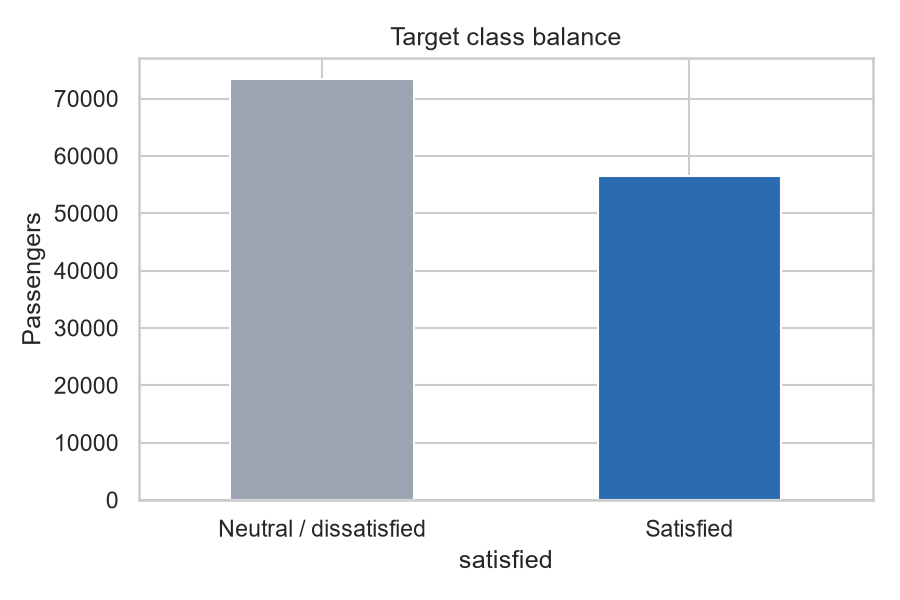
\includegraphics[width=\linewidth]{airline_class_balance.png}\caption{Class balance}\label{fig:air-balance}\end{subfigure}\hfill
\begin{subfigure}{0.62\textwidth}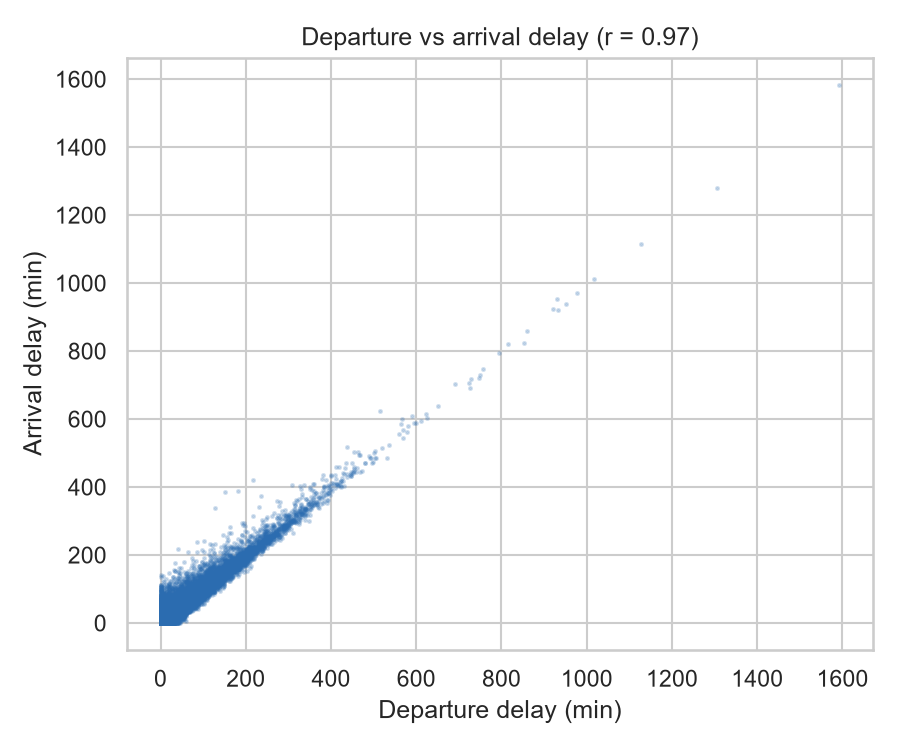
\includegraphics[width=\linewidth]{airline_delay_scatter.png}\caption{Departure vs arrival delay}\end{subfigure}
\caption{Airline target balance and delay relationship.}
\end{figure}

\begin{figure}[H]\centering
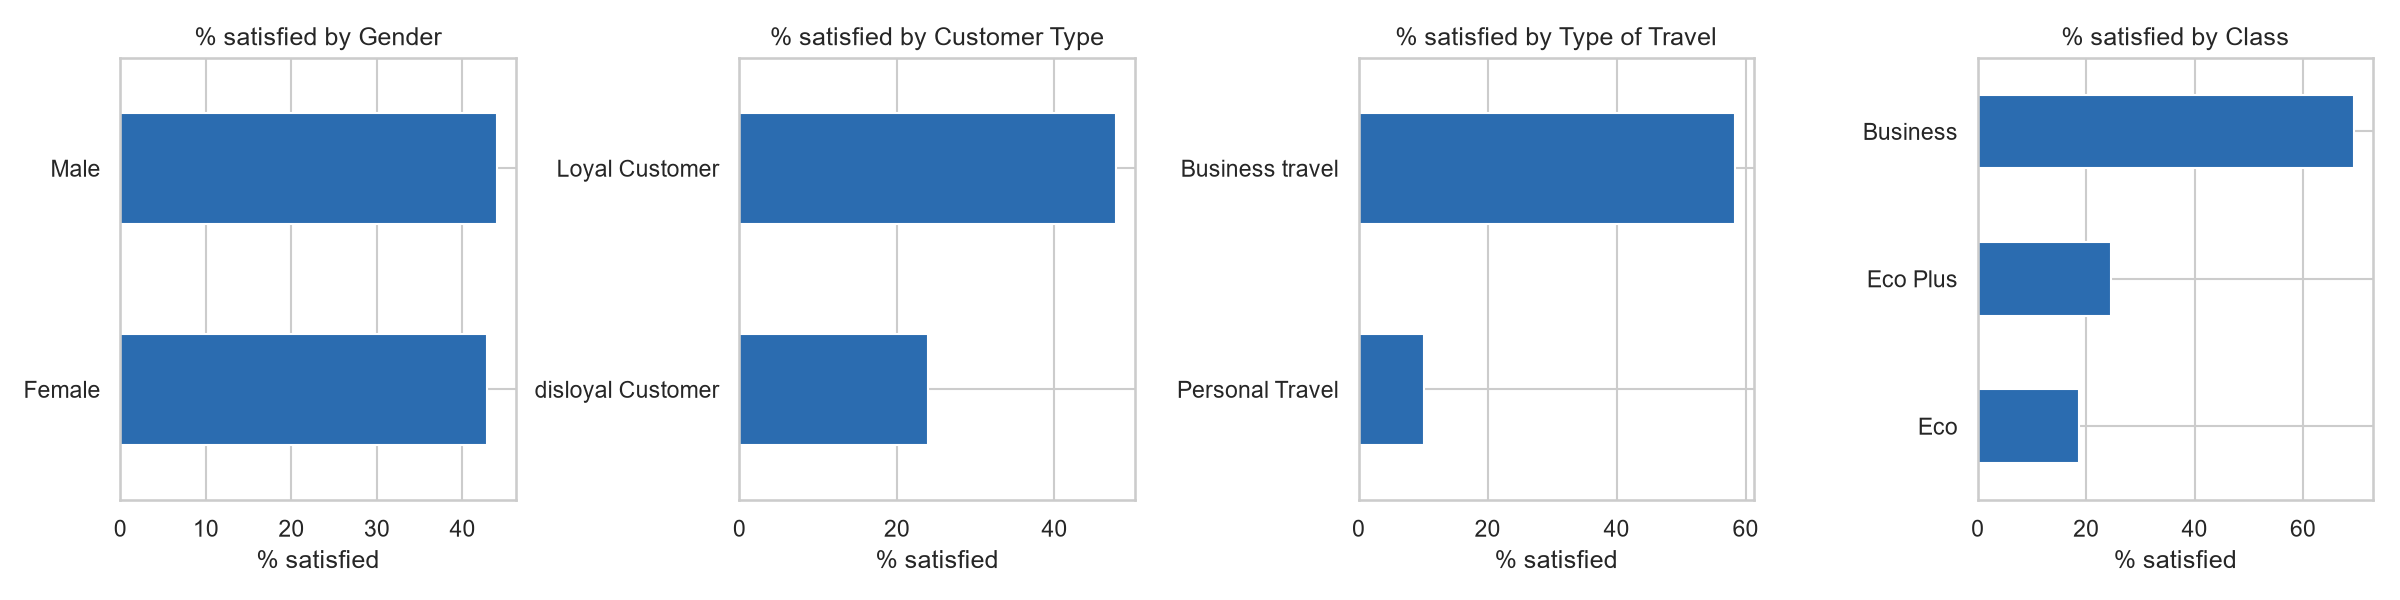
\includegraphics[width=\textwidth]{airline_categorical_vs_target.png}
\caption{Share of satisfied passengers by each categorical feature.}\label{fig:air-cat}
\end{figure}

Among the service ratings, \emph{online boarding} (r = 0.50), \emph{inflight entertainment} (0.40) and \emph{seat comfort} (0.35) correlate most with satisfaction (Figure~\ref{fig:air-corr}). Delays have a long right tail (Figures~\ref{fig:air-num} and~\ref{fig:air-box}), and departure and arrival delay are almost the same variable (r = 0.97).

\begin{figure}[H]\centering
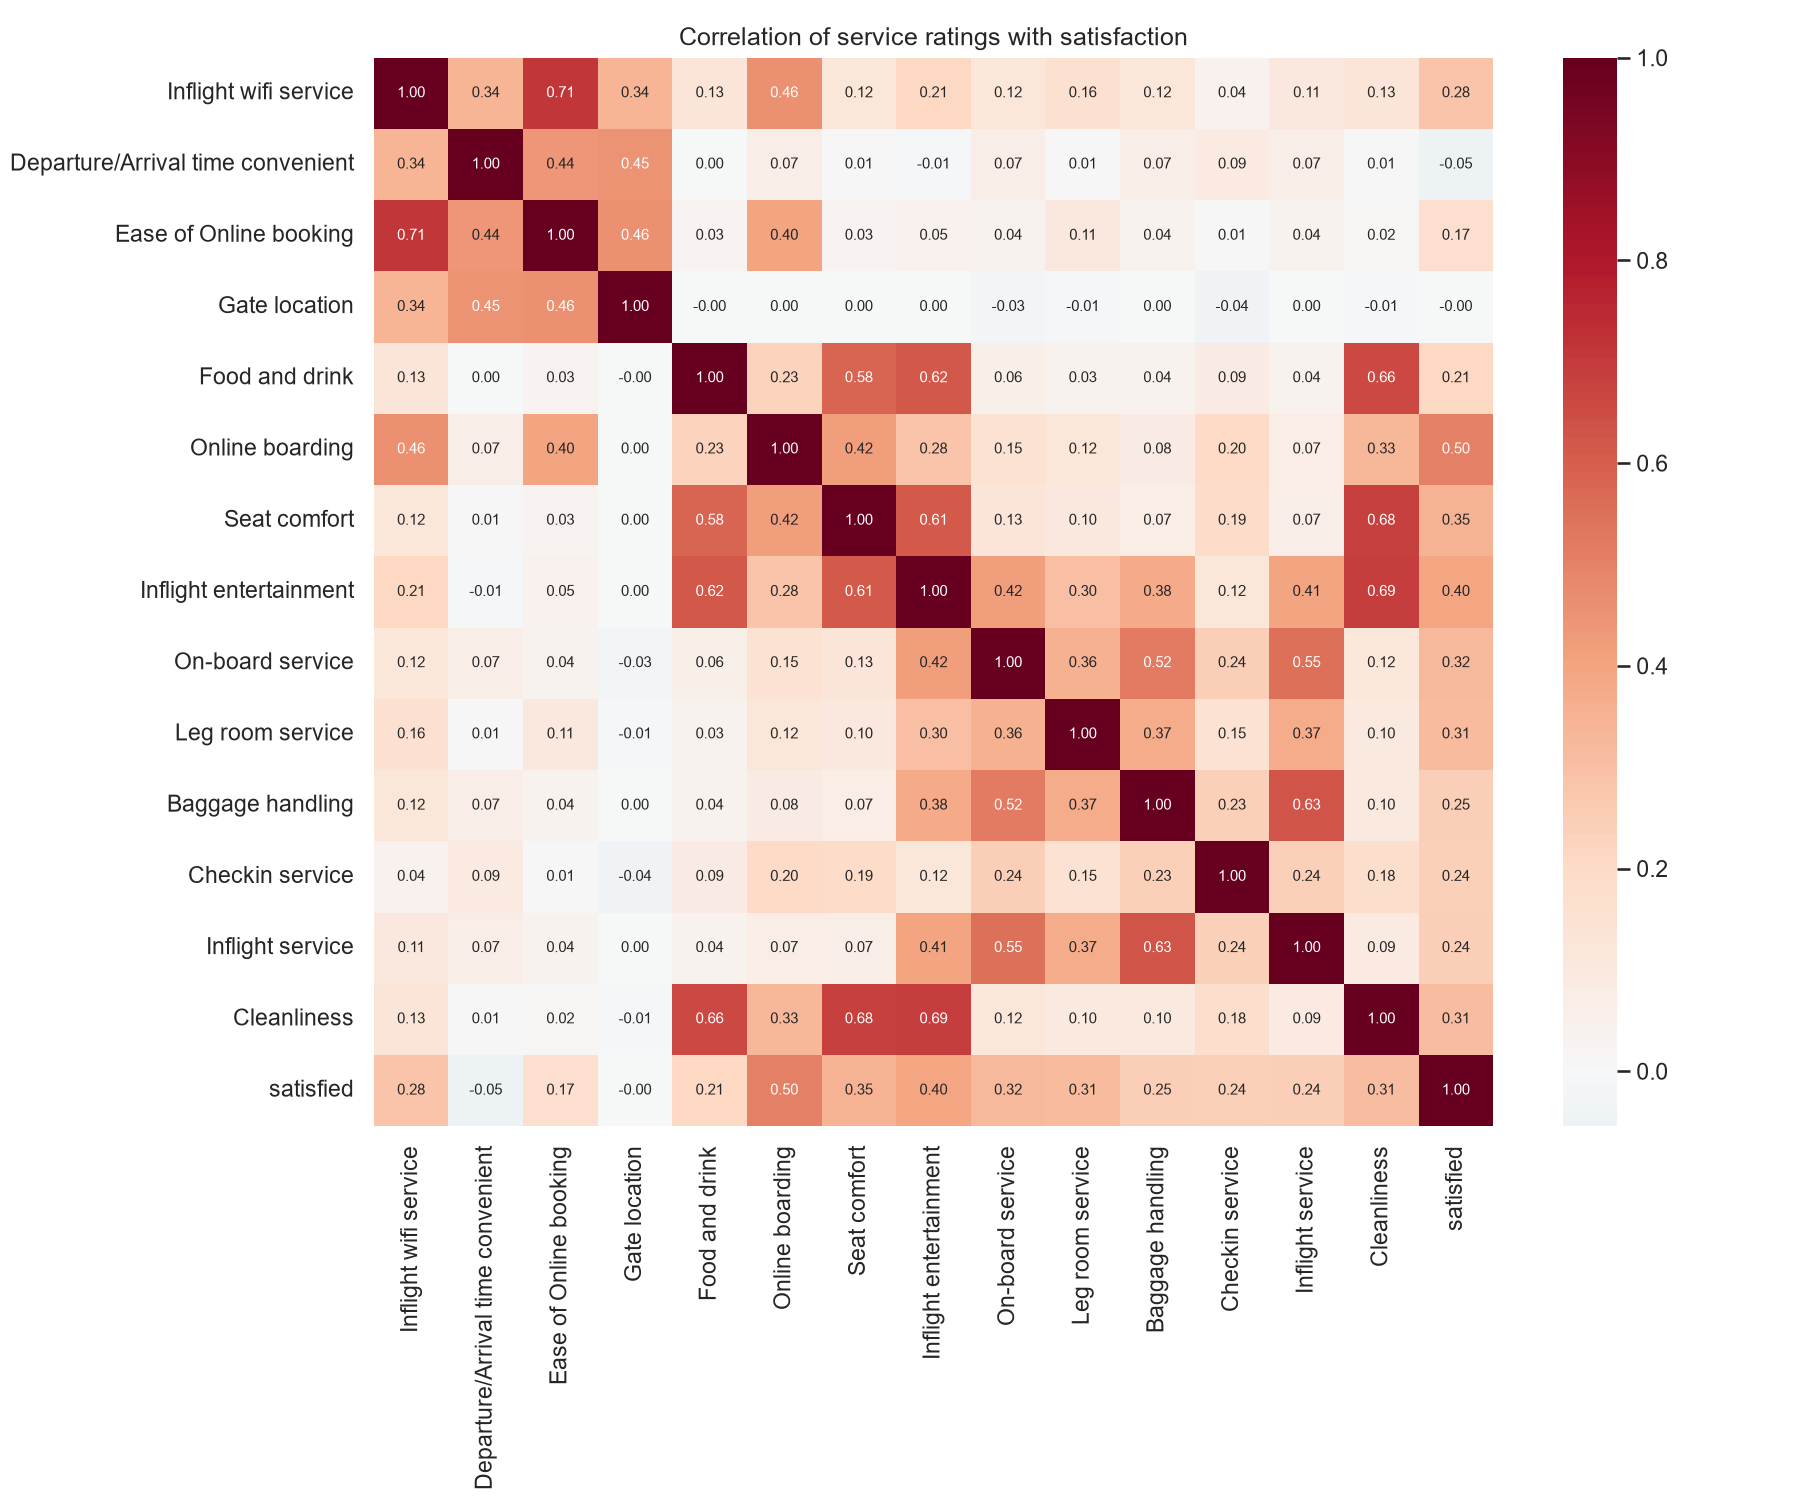
\includegraphics[width=0.78\textwidth]{airline_correlation_heatmap.png}
\caption{Correlation between service ratings and satisfaction.}\label{fig:air-corr}
\end{figure}

\begin{figure}[H]\centering
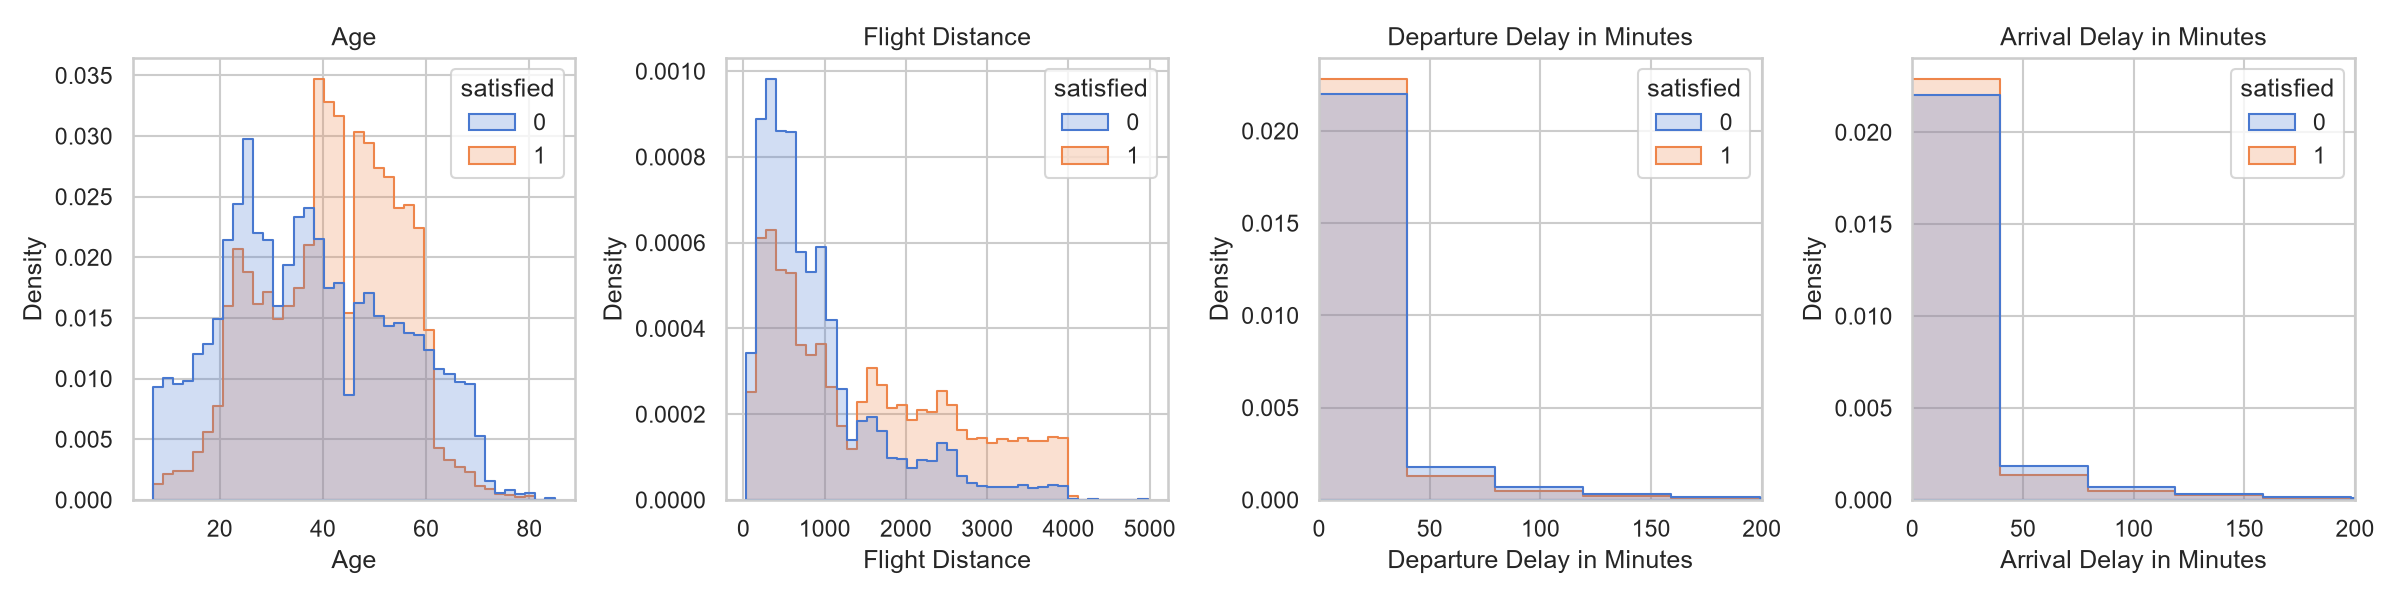
\includegraphics[width=\textwidth]{airline_numeric_distributions.png}
\caption{Numeric feature distributions by class (0 = neutral/dissatisfied, 1 = satisfied).}\label{fig:air-num}
\end{figure}

\begin{figure}[H]\centering
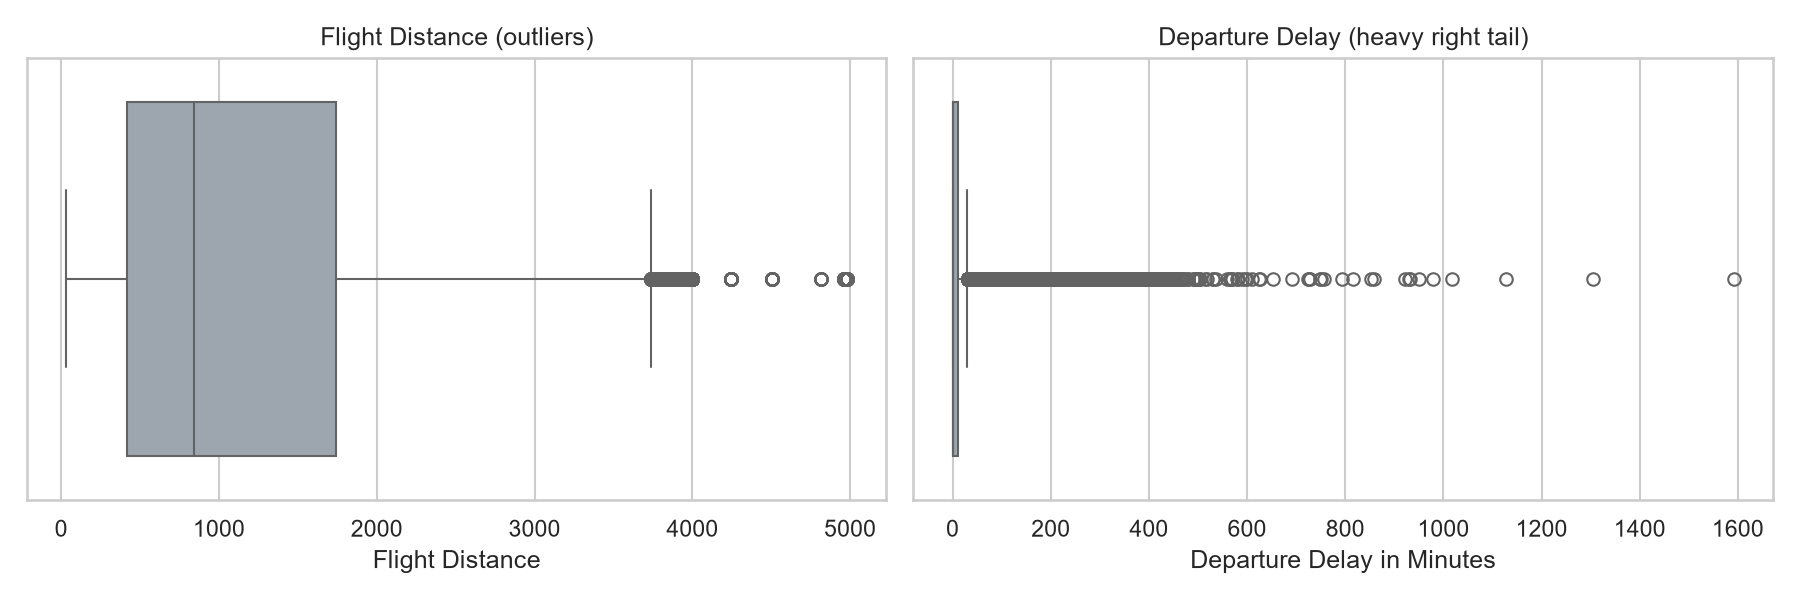
\includegraphics[width=0.9\textwidth]{airline_outliers_boxplot.png}
\caption{Outliers in flight distance and departure delay.}\label{fig:air-box}
\end{figure}

\subsection{Exploratory data analysis --- Taxi}

Trip duration is heavily right-skewed (Figure~\ref{fig:taxi-target}). The median trip is \taxiMedianMin{} minutes, but the longest lasts \taxiMaxDays{} days, and \taxiOverDay{} trips exceed 24 hours (meter errors). After a log1p transform the target is close to normal, so the model is trained on $\log(1+y)$. Minimising squared error on this scale is exactly the RMSLE metric.

\begin{figure}[H]\centering
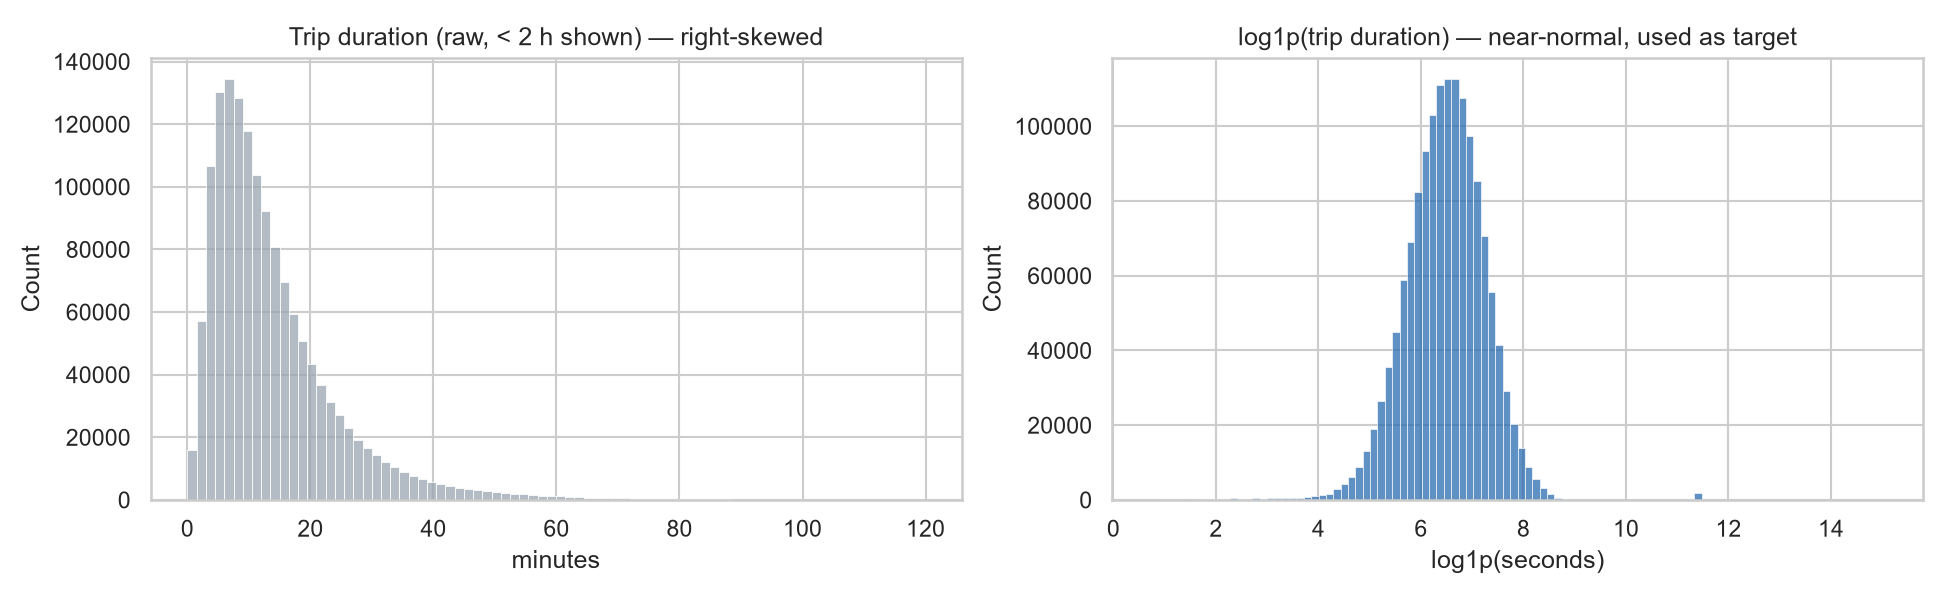
\includegraphics[width=\textwidth]{taxi_target_distribution.png}
\caption{Raw trip duration (left) and log-transformed duration (right).}\label{fig:taxi-target}
\end{figure}

Trips are longest on weekdays between 8 am and 6 pm, when traffic is heaviest (Figure~\ref{fig:taxi-heat}). Pickups concentrate in Manhattan, with visible clusters at JFK and LaGuardia airports (Figure~\ref{fig:taxi-map}). Daily volume is stable apart from a sharp drop on 23 January 2016, the day of the blizzard (Figure~\ref{fig:taxi-day}).

\begin{figure}[H]\centering
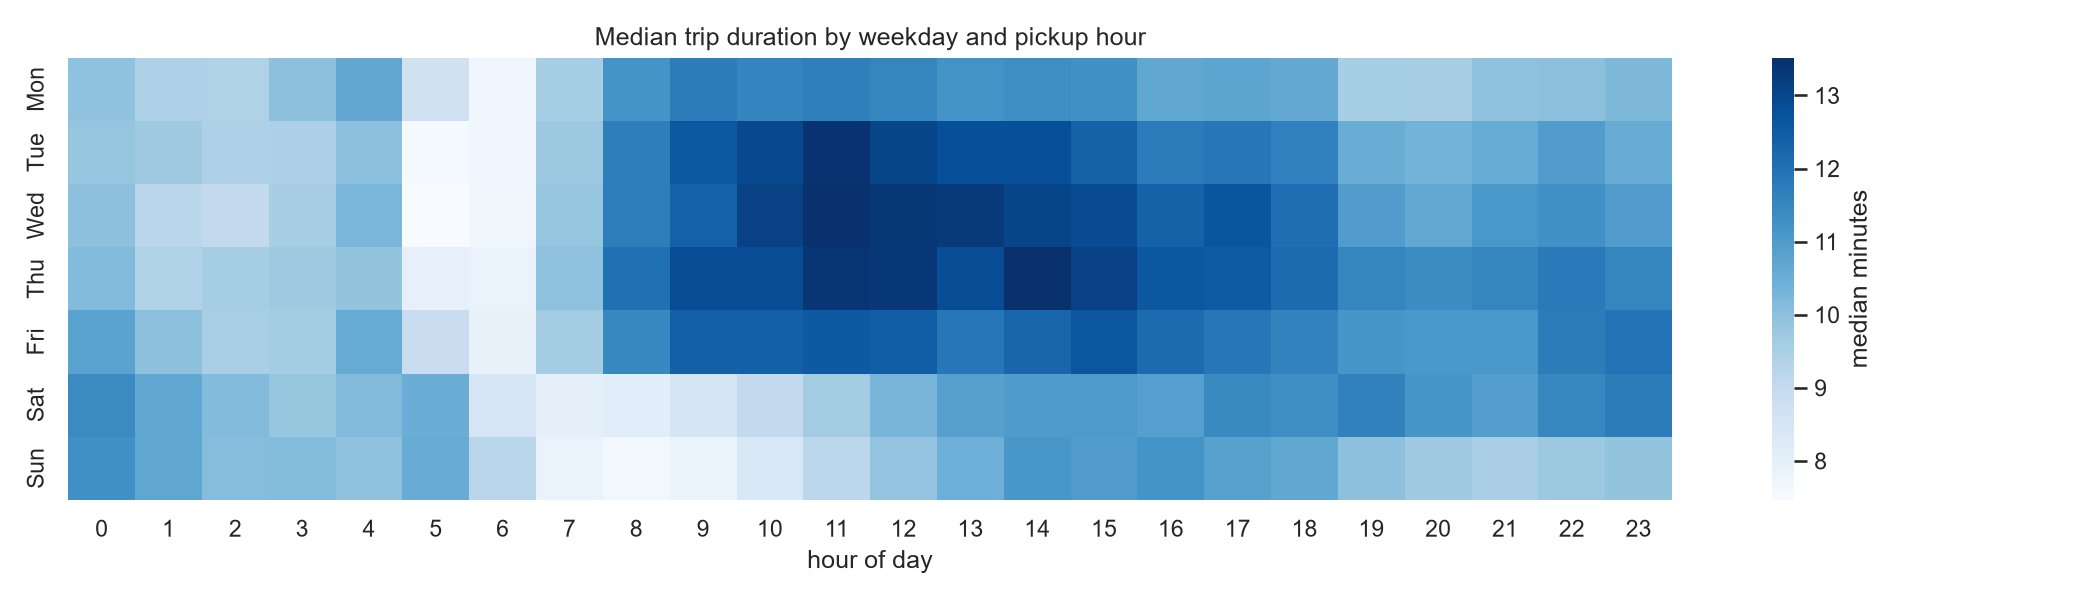
\includegraphics[width=\textwidth]{taxi_hour_weekday_heatmap.png}
\caption{Median trip duration (minutes) by weekday and pickup hour.}\label{fig:taxi-heat}
\end{figure}

\begin{figure}[H]\centering
\begin{subfigure}{0.4\textwidth}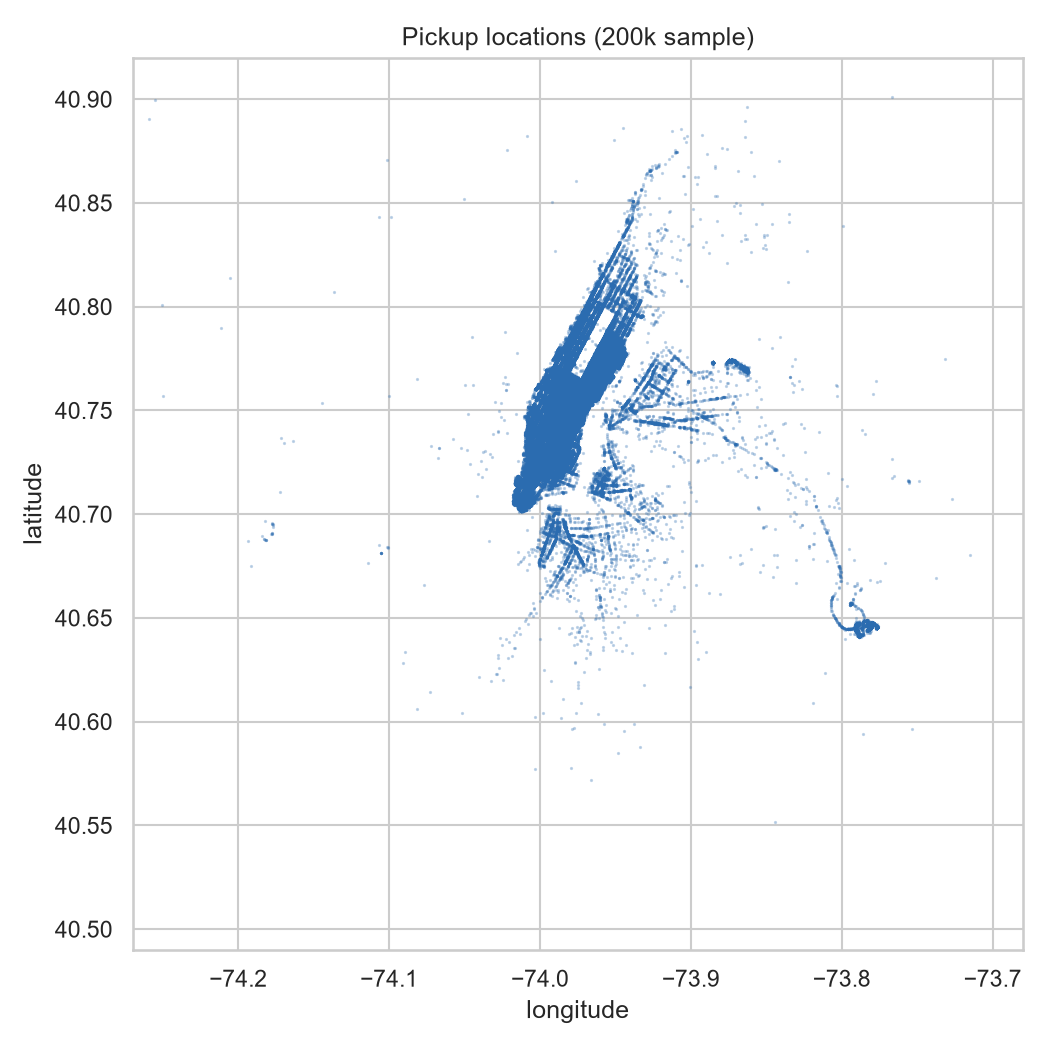
\includegraphics[width=\linewidth]{taxi_pickup_map.png}\caption{Pickup locations}\label{fig:taxi-map}\end{subfigure}\hfill
\begin{subfigure}{0.58\textwidth}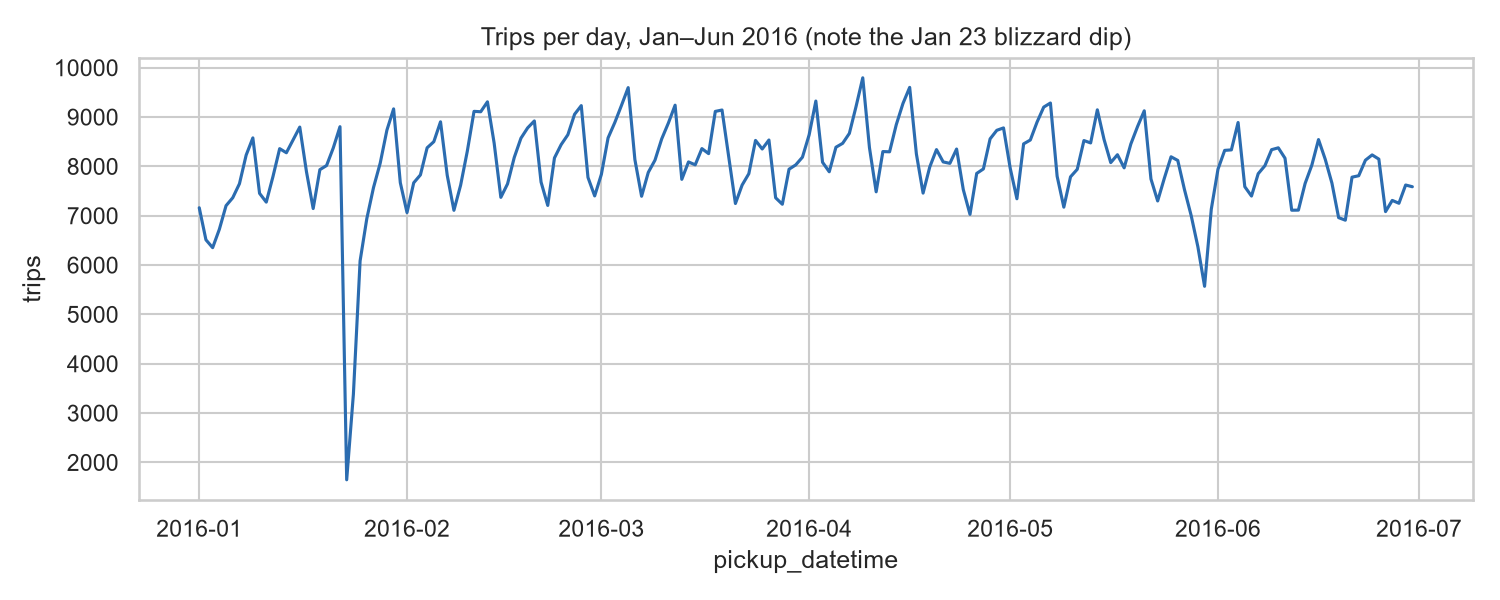
\includegraphics[width=\linewidth]{taxi_trips_per_day.png}\caption{Trips per day}\label{fig:taxi-day}\end{subfigure}
\caption{Where and when taxi trips happen.}
\end{figure}

\subsection{Data cleaning}

\begin{table}[H]\centering\small
\caption{Cleaning steps and their effect.}
\begin{tabularx}{\textwidth}{@{}p{2.6cm}LL@{}}
\toprule
Step & \textbf{Airline} & \textbf{Taxi} \\
\midrule
Missing values & \airMissing{} missing \emph{Arrival Delay} values, filled with \emph{Departure Delay} (r = 0.97) instead of dropping rows & None \\
Duplicates & 0 duplicate rows & 0 duplicate trip IDs \\
Outliers & Delays capped at the training 99.5th percentile (\airCapDep{} / \airCapArr{} min), so rows are kept but extreme values have less leverage & Removed: \taxiOutBox{} trips outside the NYC area; \taxiBadDur{} trips under 1 min or over 4 h; \taxiZeroDist{} zero-distance trips; \taxiFast{} trips with average speed $>$ 120 km/h \\
Inconsistencies & Rating 0 means \emph{not applicable}, so it is treated as missing in derived features & \taxiBadPax{} trips with 0 or more than 6 passengers removed \\
Rows kept & \airRows{} (100\%) & \taxiKept{} (\taxiRemovedPct{} removed) \\
\bottomrule
\end{tabularx}
\end{table}

\subsection{Feature engineering}

\paragraph{Airline (6 new features).} \texttt{service\_mean} (average of the 14 ratings), \texttt{service\_min} (worst rating), \texttt{low\_scores} (number of ratings $\le 2$), \texttt{total\_delay}, \texttt{delay\_gained} (arrival minus departure delay) and \texttt{log\_distance}. The four categorical features are one-hot encoded. Numeric features are standardised for Logistic Regression only, because tree models do not need scaling.

\paragraph{Taxi (27 features).}
\begin{itemize}
\item \textbf{Time:} hour, minute of day, weekday, month, day of year, weekend flag, rush-hour flag.
\item \textbf{Geometry:} haversine distance, Manhattan (L1) distance, bearing, latitude and longitude deltas, trip centre point.
\item \textbf{Places:} pickup and drop-off flags for JFK and LaGuardia airports.
\item \textbf{Unsupervised location clusters:} MiniBatch K-Means ($k=60$), fitted on training coordinates only, gives a pickup cluster and a drop-off cluster for each trip.
\end{itemize}
Figure~\ref{fig:taxi-dist} confirms that distance is the strongest single signal. Figure~\ref{fig:taxi-corr} shows each feature's linear correlation with the target.

\begin{figure}[H]\centering
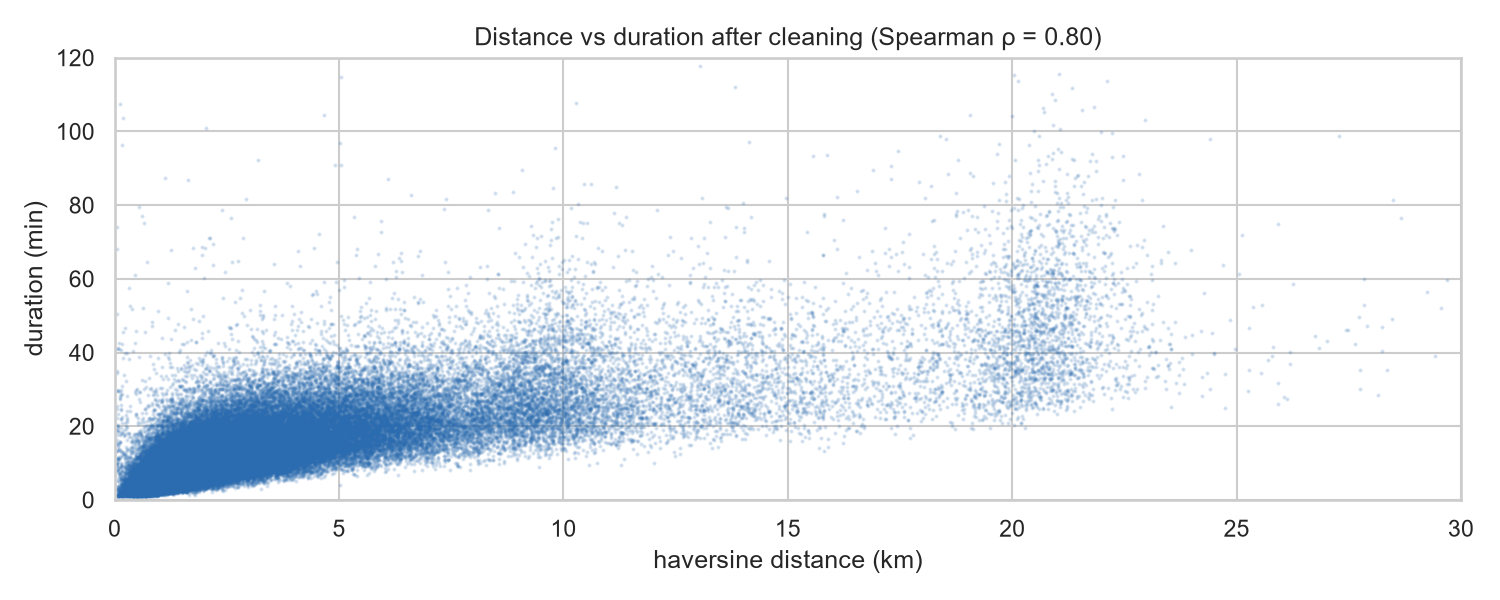
\includegraphics[width=0.85\textwidth]{taxi_distance_vs_duration.png}
\caption{Distance vs duration after cleaning.}\label{fig:taxi-dist}
\end{figure}
\begin{figure}[H]\centering
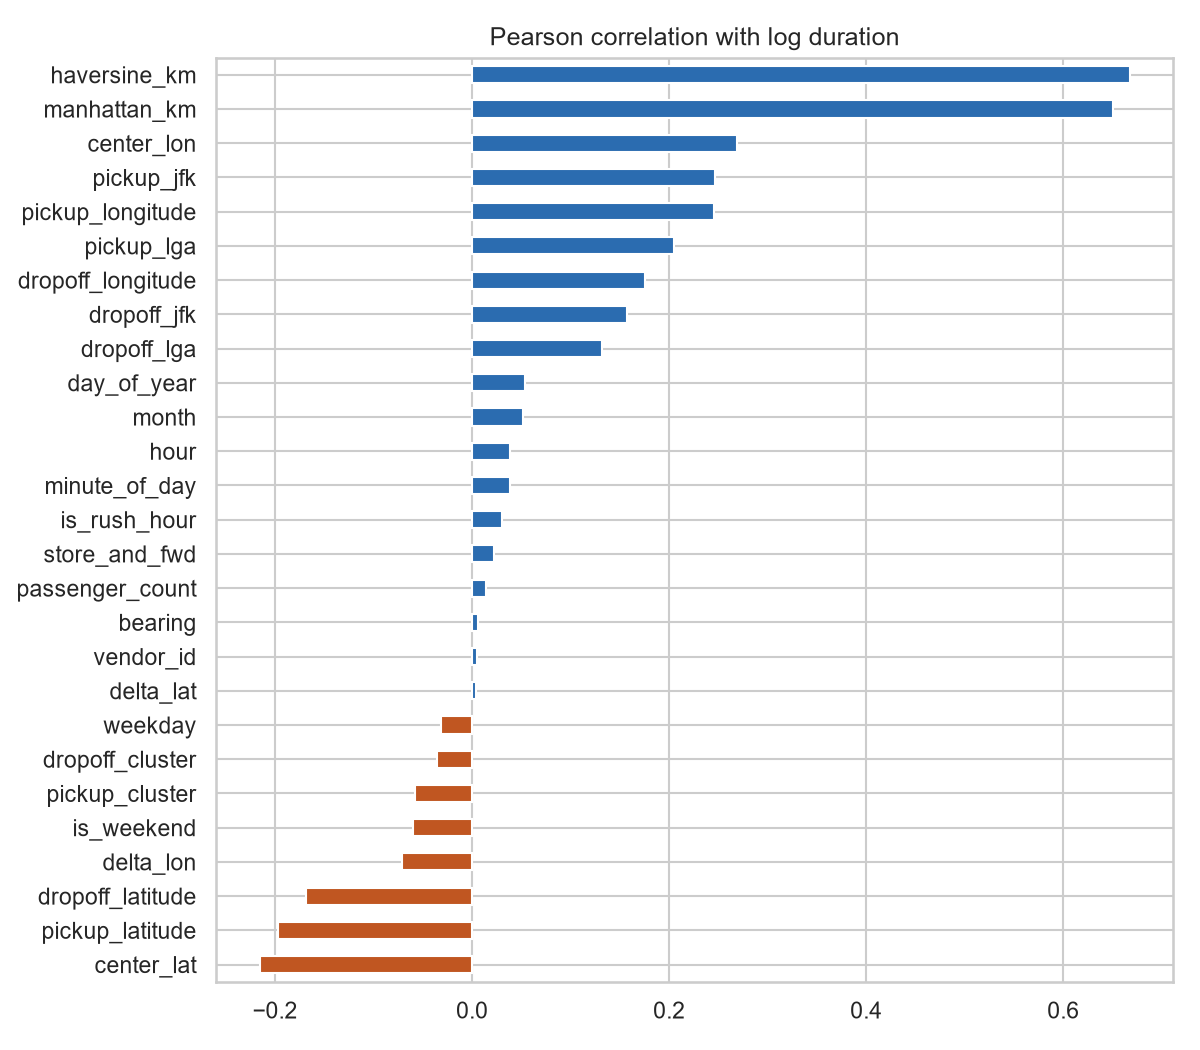
\includegraphics[width=0.62\textwidth]{taxi_feature_correlation.png}
\caption{Pearson correlation of each engineered feature with log duration.}\label{fig:taxi-corr}
\end{figure}

\subsection{Data splitting}

\begin{table}[H]\centering\small
\caption{Train / validation / test split.}
\begin{tabular}{@{}lrrrl@{}}
\toprule
 & Train & Validation & Test & Method \\
\midrule
Airline & \airTrain & \airVal & \airTest & Kaggle test file kept as test; train file split 80/20, stratified \\
Taxi & \taxiTrain & \taxiVal & \taxiTest & Random 70/15/15 split, seed 42 \\
\bottomrule
\end{tabular}
\end{table}
\noindent Imputation values, outlier caps, scalers and K-Means centres are fitted on training data only and then applied to validation and test data. This prevents information leaking from the evaluation sets into training.

%=====================================================================
\section{Algorithm Selection}

Both tasks are supervised learning on structured data, so I compared a linear baseline, a bagging ensemble and two gradient-boosting libraries. Gradient boosting was expected to perform best, because it captures non-linear effects and interactions (for example \emph{class $\times$ type of travel}, or \emph{hour $\times$ location}) without manual feature crosses. Unsupervised K-Means is also used, to build location features for the taxi model.

\begin{table}[H]\centering\small
\caption{Candidate algorithms and trade-offs.}
\begin{tabularx}{\textwidth}{@{}p{3.1cm}p{1.6cm}Lp{1.6cm}p{2.1cm}@{}}
\toprule
Algorithm & Used in & Reason & Interpret. & Compute cost \\
\midrule
Logistic Regression & Airline & Linear baseline; coefficients easy to explain & High & Very low \\
Ridge Regression & Taxi & Linear baseline with L2 regularisation & High & Very low \\
Mean prediction & Taxi & Floor every model must beat & High & None \\
Random Forest & Both & Robust non-linear ensemble, little tuning & Medium & High memory on 1M rows \\
XGBoost & Both & Regularised gradient boosting & Medium & Medium \\
LightGBM & Both & Fast histogram boosting; scales to 1M+ rows & Medium & Low--medium \\
K-Means (k = 60) & Taxi features & Groups coordinates into neighbourhoods & High & Low \\
\bottomrule
\end{tabularx}
\end{table}

\noindent Neural networks were not used. On tabular data of this size, boosted trees usually match or beat them at a fraction of the tuning cost, and they are easier to explain. Reinforcement learning does not apply, because neither problem involves sequential decisions.

%=====================================================================
\section{Model Development and Training}

Every model is a scikit-learn \texttt{Pipeline}, so preprocessing and model are saved together and the same code runs in training and in deployment. Each project has one script that runs all the steps and saves metrics (JSON), figures (PNG) and the final model (\texttt{joblib}):
\begin{lstlisting}
python src/airline_pipeline.py
python src/taxi_pipeline.py
\end{lstlisting}
\noindent On an 8-core laptop the airline script runs in \airRuntime{} minutes and the taxi script in \taxiRuntime{} minutes.

\noindent\textbf{Airline:} \texttt{ColumnTransformer} (median imputer, \texttt{StandardScaler} for the linear model, \texttt{OneHotEncoder}) followed by the classifier. Starting settings: Logistic Regression (C = 1); Random Forest (300 trees); XGBoost (400 trees, learning rate 0.1, depth 6); LightGBM (400 trees, learning rate 0.05, 31 leaves).

\noindent\textbf{Taxi:} the shared \texttt{add\_features()} function, followed by the regressor, trained on $\log(1+y)$. Starting settings: Ridge ($\alpha$ = 1, standardised); Random Forest (150 trees, min leaf 5, trained on a 200k-row sample because of memory); XGBoost (600 trees, learning rate 0.1, depth 8, \texttt{hist}); LightGBM (600 trees, learning rate 0.1, 127 leaves). All runs use random seed 42.

%=====================================================================
\section{Model Evaluation and Hyperparameter Tuning}

\subsection{Validation results and over/underfitting}

\begin{table}[H]\centering\small
\caption{Airline --- baseline models (validation set, \airVal{} passengers).}
\begin{tabular}{@{}lrrrrrrr@{}}
\toprule
Model & Train acc. & Val acc. & Precision & Recall & F1 & ROC-AUC & Fit (s) \\
\midrule
Logistic Regression & \airLogisticRegressionTraAccuracy & \airLogisticRegressionValAccuracy & \airLogisticRegressionValPrecision & \airLogisticRegressionValRecall & \airLogisticRegressionValF & \airLogisticRegressionValRocAuc & \airLogisticRegressionFit \\
Random Forest & \airRandomForestTraAccuracy & \airRandomForestValAccuracy & \airRandomForestValPrecision & \airRandomForestValRecall & \airRandomForestValF & \airRandomForestValRocAuc & \airRandomForestFit \\
XGBoost & \airXgboostTraAccuracy & \airXgboostValAccuracy & \airXgboostValPrecision & \airXgboostValRecall & \airXgboostValF & \airXgboostValRocAuc & \airXgboostFit \\
LightGBM & \airLightgbmTraAccuracy & \airLightgbmValAccuracy & \airLightgbmValPrecision & \airLightgbmValRecall & \airLightgbmValF & \airLightgbmValRocAuc & \airLightgbmFit \\
\midrule
\textbf{LightGBM (tuned)} & \airTunedTrAccuracy & \textbf{\airTunedValAccuracy} & \airTunedValPrecision & \airTunedValRecall & \textbf{\airTunedValF} & \textbf{\airTunedValRocAuc} & --- \\
\bottomrule
\end{tabular}
\end{table}

\begin{itemize}
\item \textbf{Underfitting:} Logistic Regression scores the same on train and validation (\airLogisticRegressionTraAccuracy{} vs \airLogisticRegressionValAccuracy). Both are low, so a linear boundary is too simple for this data.
\item \textbf{Overfitting:} Random Forest memorises the training set (train accuracy \airRandomForestTraAccuracy) and loses \airRandomForestGap{} points on validation.
\item \textbf{Good fit:} LightGBM has the best validation scores with a gap of only \airLightgbmGap{} points, so it was chosen for tuning.
\end{itemize}

\begin{figure}[H]\centering
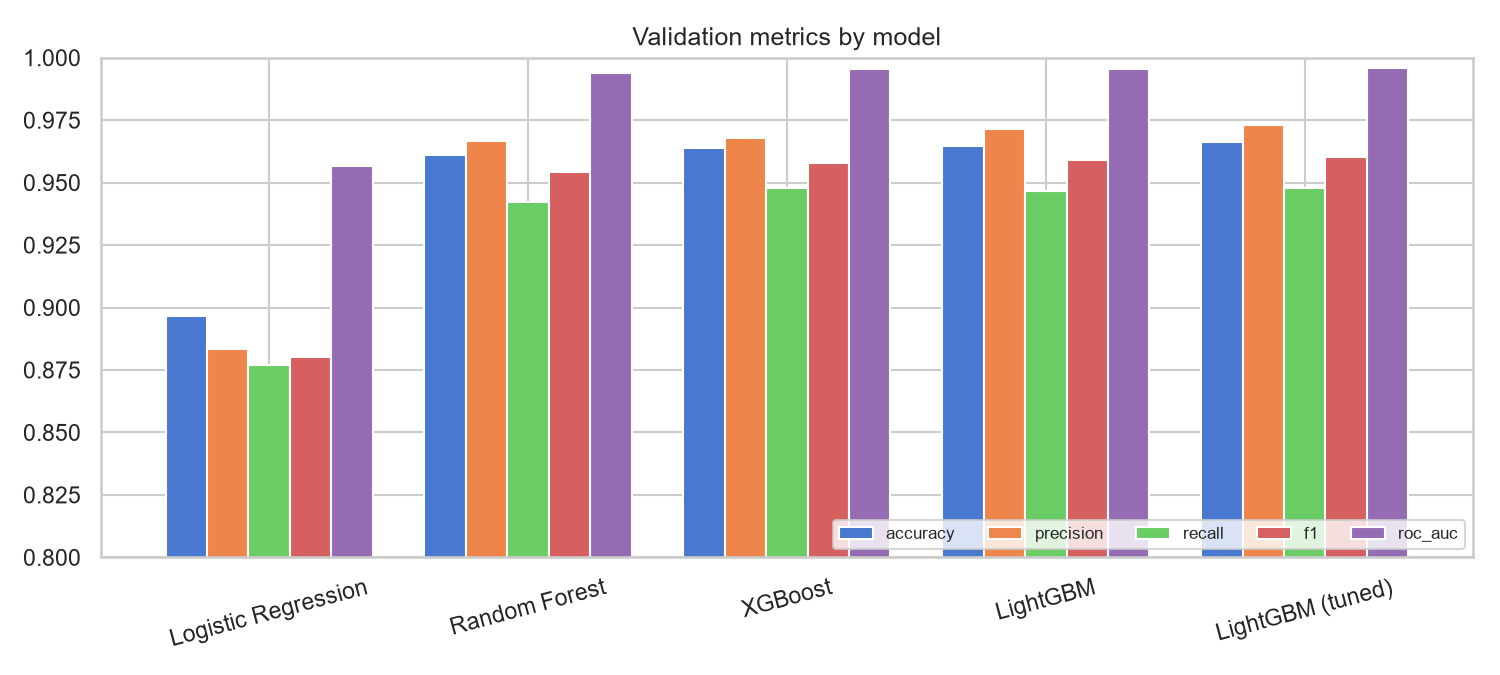
\includegraphics[width=0.9\textwidth]{airline_model_comparison.png}
\caption{Airline validation metrics by model.}
\end{figure}

\begin{table}[H]\centering\small
\caption{Taxi --- baseline models (validation set, \taxiVal{} trips). MAE in minutes.}
\begin{tabular}{@{}lrrrrr@{}}
\toprule
Model & Train RMSLE & Val RMSLE & Val $R^2$ (log) & Val MAE (min) & Fit (s) \\
\midrule
Mean baseline & \taxiMeanBaselineTraRmsle & \taxiMeanBaselineValRmsle & \taxiMeanBaselineValRLog & \taxiMeanBaselineValMaeSeconds & --- \\
Ridge Regression & \taxiRidgeRegressionTraRmsle & \taxiRidgeRegressionValRmsle & \taxiRidgeRegressionValRLog & \taxiRidgeRegressionValMaeSeconds & \taxiRidgeRegressionFit \\
Random Forest (200k) & \taxiRandomForestTraRmsle & \taxiRandomForestValRmsle & \taxiRandomForestValRLog & \taxiRandomForestValMaeSeconds & \taxiRandomForestFit \\
XGBoost & \taxiXgboostTraRmsle & \taxiXgboostValRmsle & \taxiXgboostValRLog & \taxiXgboostValMaeSeconds & \taxiXgboostFit \\
LightGBM & \taxiLightgbmTraRmsle & \taxiLightgbmValRmsle & \taxiLightgbmValRLog & \taxiLightgbmValMaeSeconds & \taxiLightgbmFit \\
\midrule
\textbf{LightGBM (tuned)} & \taxiTunedTrRmsle & \textbf{\taxiTunedValRmsle} & \textbf{\taxiTunedValRLog} & --- & --- \\
\bottomrule
\end{tabular}
\end{table}

\noindent Ridge underfits (RMSLE \taxiRidgeRegressionValRmsle), because duration is not linear in coordinates and time. The tree ensembles roughly halve the error of the mean baseline. LightGBM is the most accurate and among the fastest, so it was tuned.

\begin{figure}[H]\centering
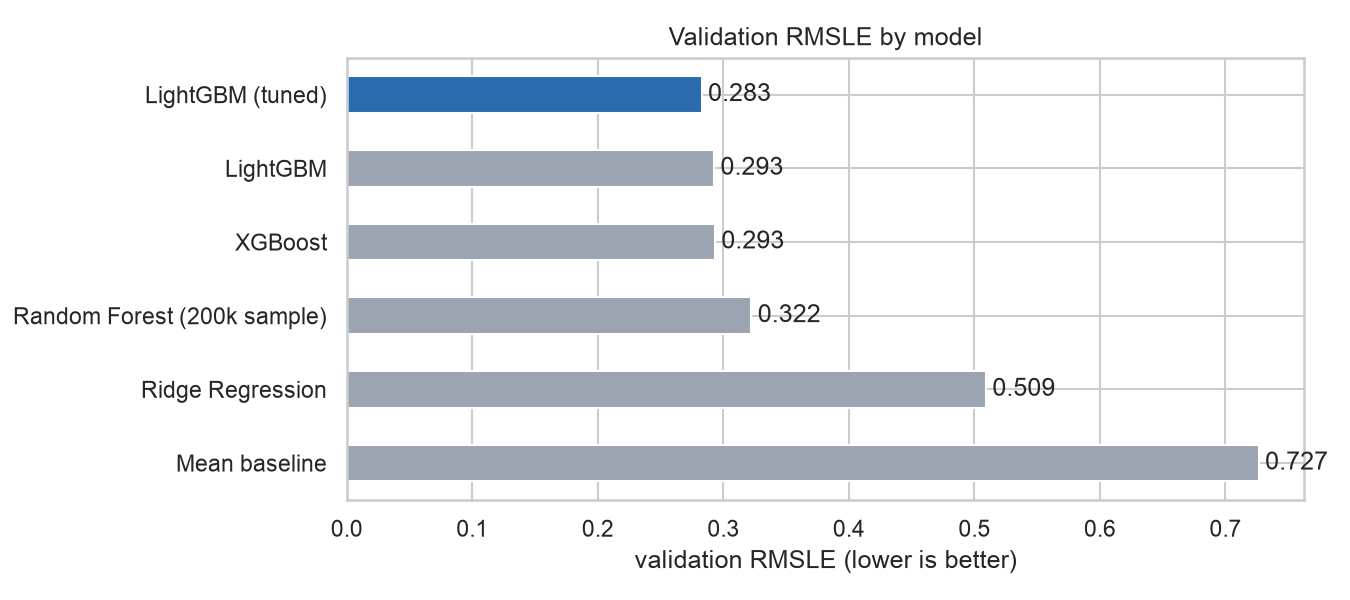
\includegraphics[width=0.8\textwidth]{taxi_model_comparison.png}
\caption{Taxi validation RMSLE by model (lower is better).}
\end{figure}

\subsection{Hyperparameter tuning}

Two search strategies from the assignment were used:
\begin{itemize}
\item \textbf{Grid search} for the linear models, which have small discrete search spaces. Airline Logistic Regression over C $\in \{0.01, 0.1, 1, 10\}$, 5-fold CV: best C = \airLrBestC{}, CV F1 \airLrCvFone. Taxi Ridge over $\alpha \in \{0.01,\dots,100\}$, 3-fold CV: best $\alpha$ = \taxiRidgeAlpha{}, CV RMSLE \taxiRidgeCv.
\item \textbf{Random search} for LightGBM, whose space is large and continuous: learning rate (log-uniform), number of trees, leaves, minimum child samples, row and column subsampling, and L2 regularisation.
\end{itemize}

\begin{table}[H]\centering\small
\caption{Best LightGBM hyperparameters found by random search.}
\begin{tabular}{@{}lrr@{}}
\toprule
Hyperparameter & Airline (25 trials, 5-fold CV) & Taxi (15 trials, 3-fold CV, 300k rows) \\
\midrule
learning\_rate & \airBpLearningRate & \taxiBpLearningRate \\
n\_estimators & \airBpNEstimators & \taxiBestIter{} (cap; early stopping not triggered) \\
num\_leaves & \airBpNumLeaves & \taxiBpNumLeaves \\
min\_child\_samples & \airBpMinChildSamples & \taxiBpMinChildSamples \\
subsample & \airBpSubsample & \taxiBpSubsample \\
colsample\_bytree & \airBpColsampleBytree & \taxiBpColsampleBytree \\
reg\_lambda & \airBpRegLambda & \taxiBpRegLambda \\
\midrule
CV score & F1 = \airLgbCvFone & RMSLE = \taxiLgbCv \\
\bottomrule
\end{tabular}
\end{table}

\noindent For the taxi model, the tuned parameters were refit on all \taxiTrain{} training rows with up to 4{,}000 trees and early stopping (patience 100) on the validation set. Validation error was still falling slowly at the cap, so all \taxiBestIter{} trees were kept (Figure~\ref{fig:taxi-lc}). More trees would give only marginal gains at a higher training cost. The final train vs validation RMSLE (\taxiTunedTrRmsle{} vs \taxiTunedValRmsle) shows mild, acceptable overfitting.

\begin{figure}[H]\centering
\begin{subfigure}{0.49\textwidth}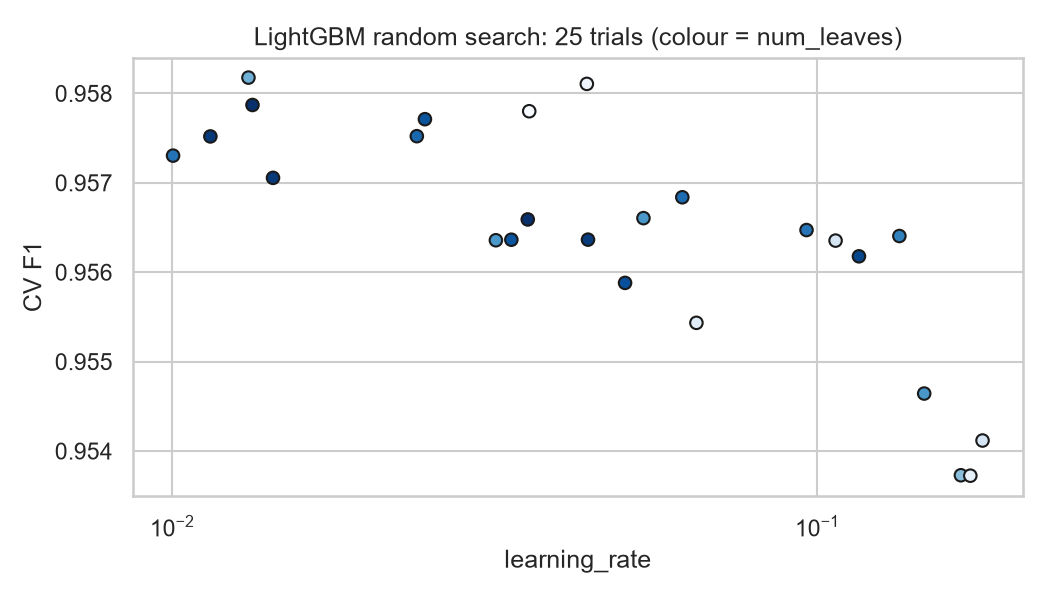
\includegraphics[width=\linewidth]{airline_random_search.png}\caption{Airline random search}\end{subfigure}\hfill
\begin{subfigure}{0.49\textwidth}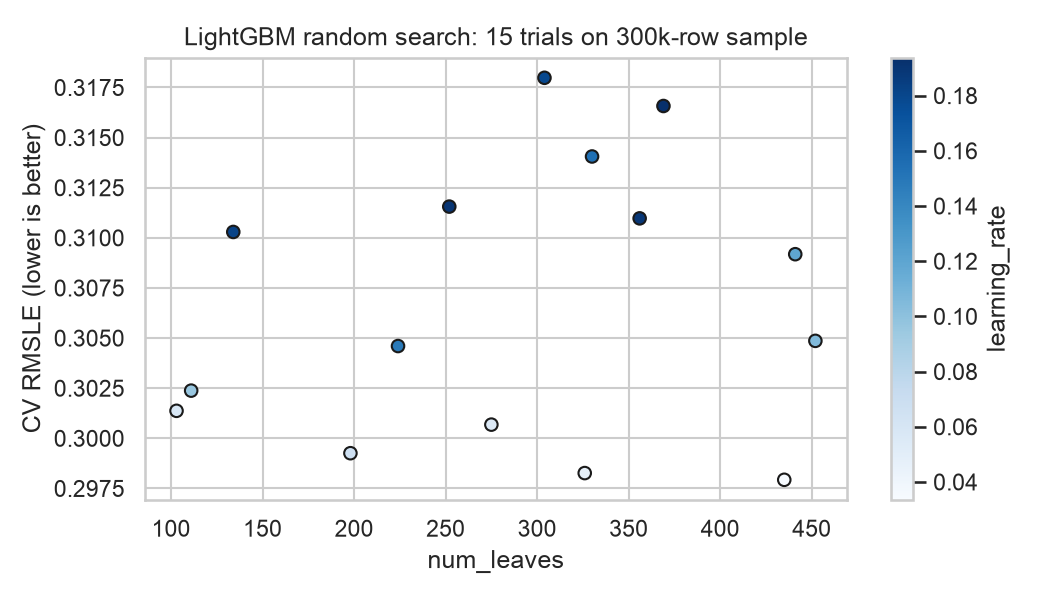
\includegraphics[width=\linewidth]{taxi_random_search.png}\caption{Taxi random search}\end{subfigure}
\caption{Random search trials for LightGBM.}
\end{figure}
\begin{figure}[H]\centering
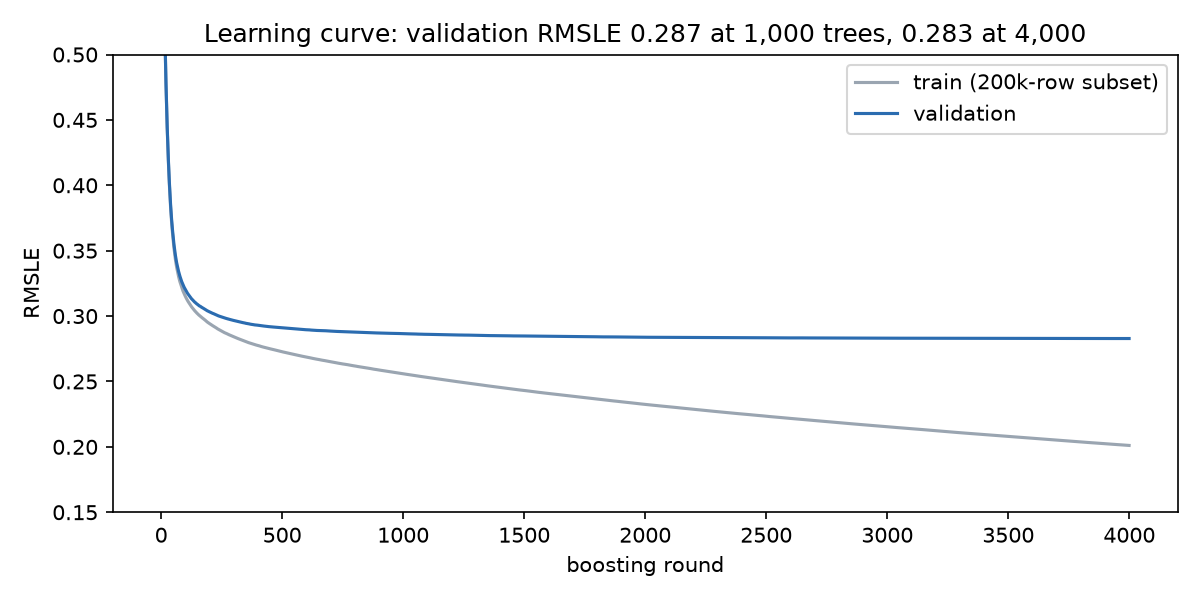
\includegraphics[width=0.7\textwidth]{taxi_learning_curve.png}
\caption{Taxi LightGBM learning curve on the log scale. Validation error flattens after about 1{,}000 trees.}\label{fig:taxi-lc}
\end{figure}

%=====================================================================
\section{Model Testing and Deployment}

\subsection{Final test results}

Each final model was evaluated once on its held-out test set, which was not used for any training or tuning decision. The airline model was refit on train + validation before testing.

\begin{table}[H]\centering\small
\caption{Test-set results against the success criteria.}
\begin{tabular}{@{}llll@{}}
\toprule
Project & Metric & Target & \textbf{Result} \\
\midrule
Airline & Accuracy & $\ge 0.95$ & \textbf{\airTestAccuracy} \\
 & Precision / Recall & --- & \airTestPrecision{} / \airTestRecall \\
 & F1-score & $\ge 0.94$ & \textbf{\airTestF} \\
 & ROC-AUC & $\ge 0.98$ & \textbf{\airTestRocAuc} \\
\midrule
Taxi & RMSLE & $\le 0.40$ & \textbf{\taxiTestRmsle} \\
 & $R^2$ (log duration) & $\ge 0.70$ & \textbf{\taxiTestRtwoLog} \\
 & $R^2$ (seconds) & --- & \taxiTestRtwoSec \\
 & MAE / median AE & --- & \taxiTestMaeMin{} min / \taxiTestMedAeMin{} min \\
 & RMSE & --- & \taxiTestRmseMin{} min \\
\bottomrule
\end{tabular}
\end{table}
\noindent Test scores are almost identical to validation scores for both projects, so the models generalise well to unseen data.

\begin{figure}[H]\centering
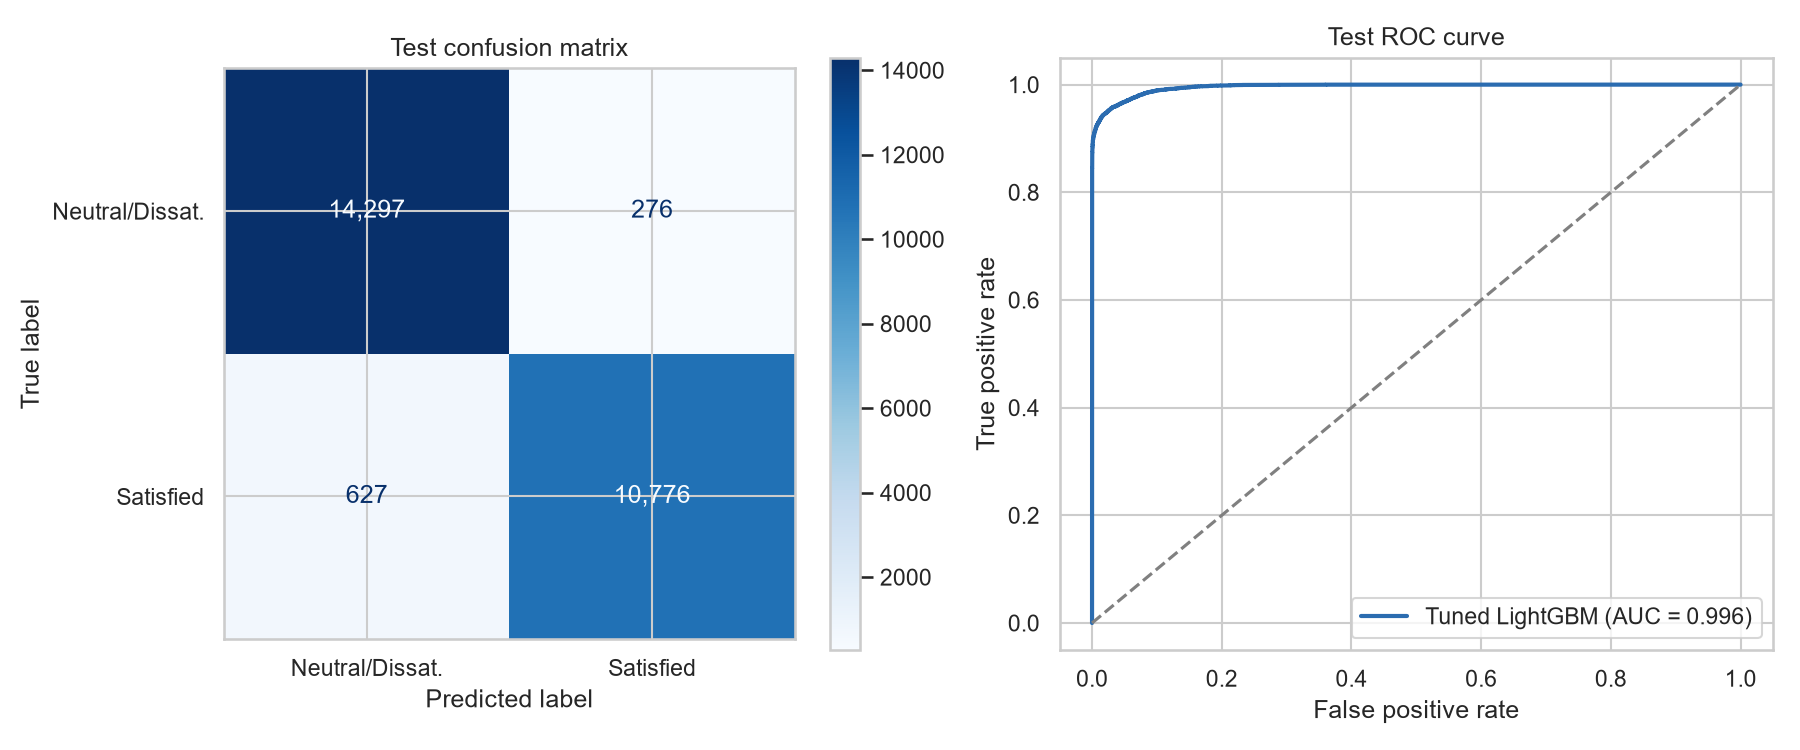
\includegraphics[width=\textwidth]{airline_test_confusion_roc.png}
\caption{Airline test confusion matrix and ROC curve.}
\end{figure}
\begin{figure}[H]\centering
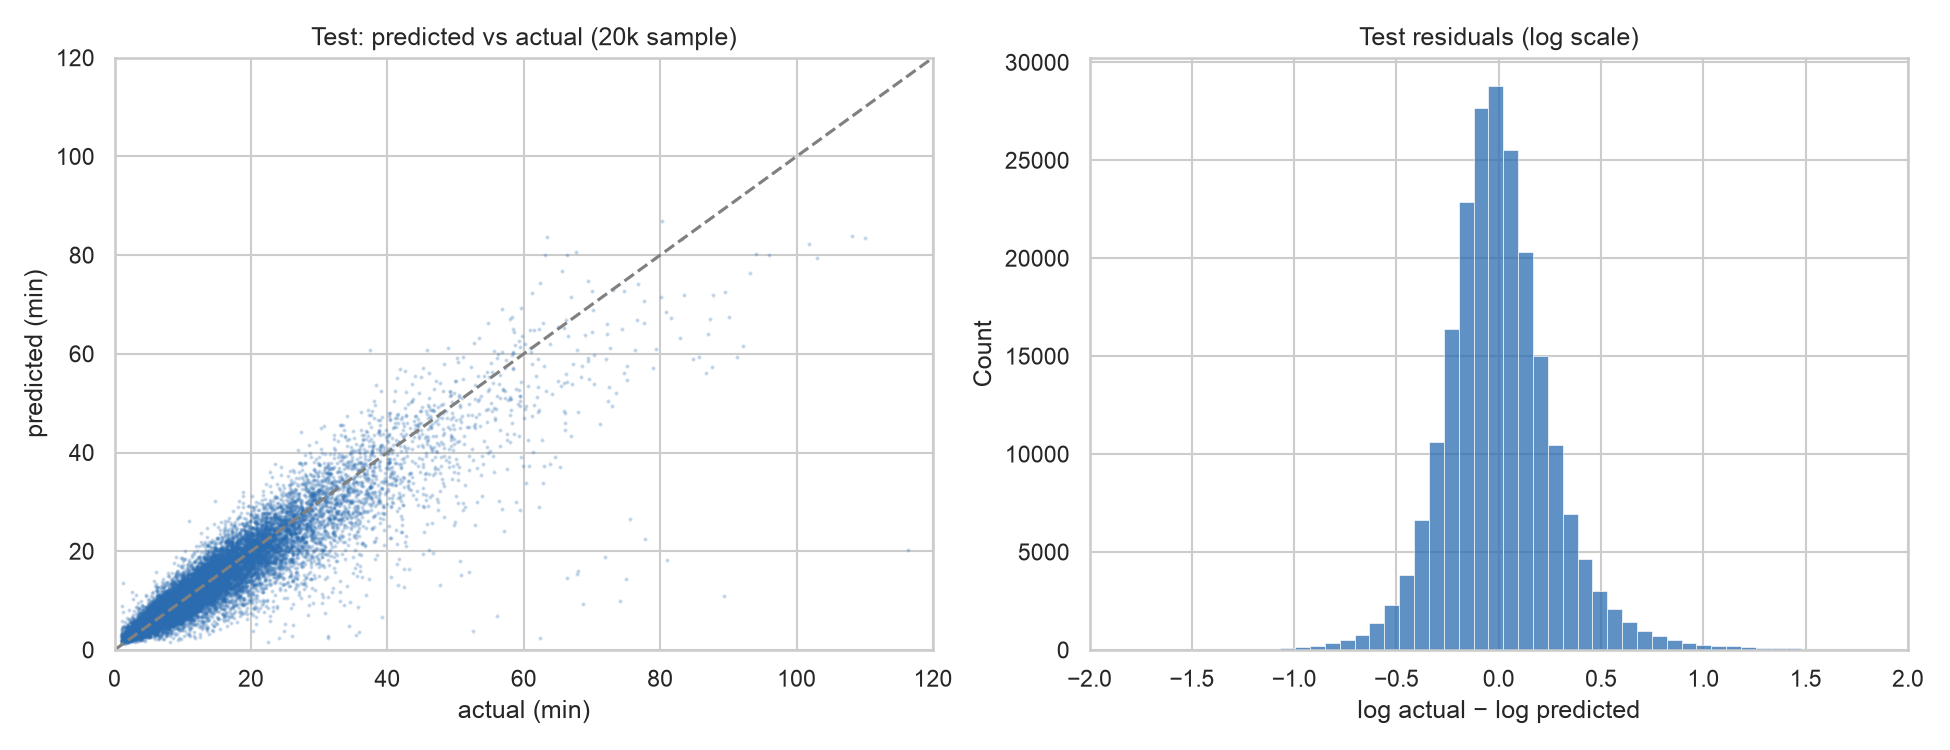
\includegraphics[width=\textwidth]{taxi_test_pred_vs_actual.png}
\caption{Taxi test predictions vs actual durations, and residuals on the log scale.}
\end{figure}

\subsection{Model interpretation}

\begin{figure}[H]\centering
\begin{subfigure}{0.49\textwidth}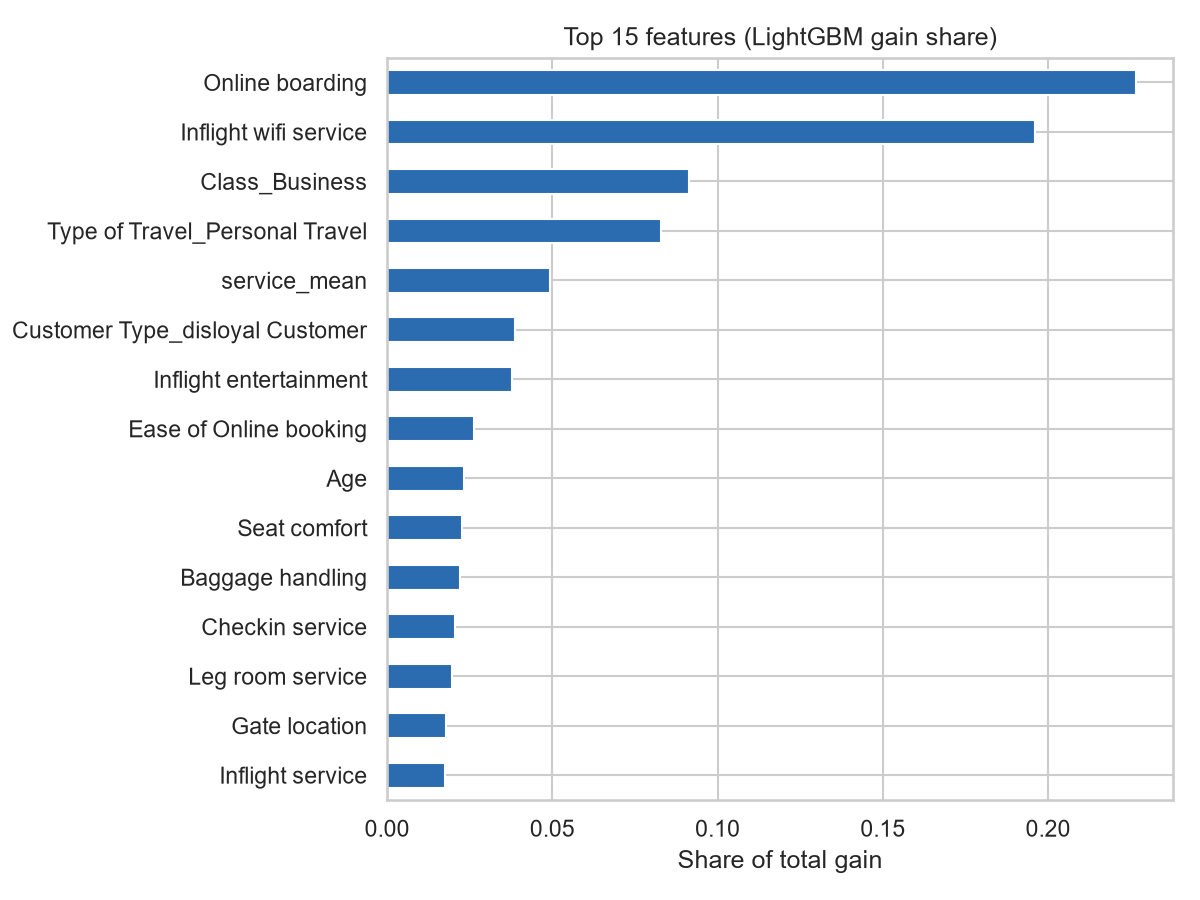
\includegraphics[width=\linewidth]{airline_feature_importance.png}\caption{Airline}\end{subfigure}\hfill
\begin{subfigure}{0.49\textwidth}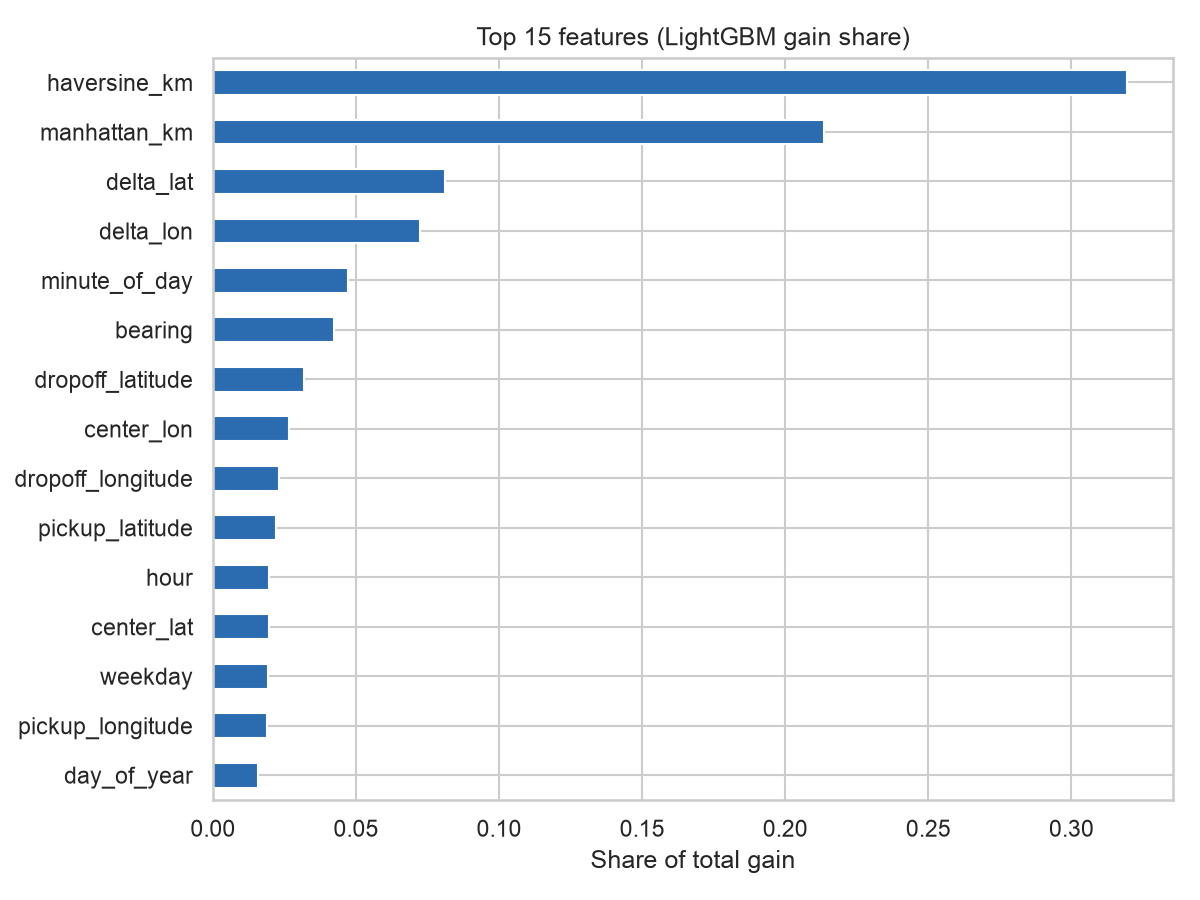
\includegraphics[width=\linewidth]{taxi_feature_importance.png}\caption{Taxi}\end{subfigure}
\caption{Top 15 features by LightGBM gain.}
\end{figure}

\noindent\textbf{Airline:} online boarding and inflight wifi together carry \airTopShare{} of the model's gain, followed by Business class and type of travel. The recommendation is to fix the digital journey first, then target economy and personal-travel passengers.
\textbf{Taxi:} distance features dominate. Engineered geometry (Manhattan distance, coordinate deltas, bearing, trip centre) and time of day refine the estimate. The K-Means clusters and airport flags add little beyond the raw coordinates, so they do not reach the top 15. The remaining error mostly comes from traffic and events that the data does not record.

\subsection{Deployment}

The saved models are served in two ways. Both use \texttt{src/inference.py}, which applies exactly the same cleaning and feature engineering as training.
\begin{itemize}
\item \textbf{Streamlit web app} (\texttt{app/streamlit\_app.py}): one tab per model with input forms, a map of the taxi route, predicted probability or duration, inference latency, and a feedback form.
\item \textbf{FastAPI REST service} (\texttt{api/main.py}): \texttt{POST /predict/airline}, \texttt{POST /predict/taxi}, \texttt{GET /monitoring} and \texttt{GET /health}. Pydantic schemas validate the inputs (for example age 1--100, ratings 0--5, coordinates inside NYC), and invalid requests return HTTP 422.
\end{itemize}
\begin{lstlisting}
streamlit run app/streamlit_app.py           # http://localhost:8501
uvicorn api.main:app --port 8000             # http://localhost:8000/docs
curl -X POST localhost:8000/predict/taxi -H 'Content-Type: application/json' \
  -d '{"pickup_datetime":"2016-04-12T17:30:00","pickup_latitude":40.758,
       "pickup_longitude":-73.9855,"dropoff_latitude":40.6413,
       "dropoff_longitude":-73.7781,"passenger_count":1,"vendor_id":2}'
\end{lstlisting}
\noindent Single-row inference takes \airLatP{} ms (airline) and \taxiLatP{} ms (taxi) at the median. For free cloud hosting, the repository can be connected to Streamlit Community Cloud with \texttt{app/streamlit\_app.py} as the entry point; the README lists the steps.

%=====================================================================
\section{Monitoring and Maintenance}

\texttt{src/monitor.py} simulates production use. It sends 500 held-out airline passengers and 500 taxi trips from \emph{June 2016}, the most recent month, through the API, then checks three things:
\begin{enumerate}
\item \textbf{Response latency.} Every request is logged to \texttt{logs/requests.jsonl}, and p50/p95/p99 latency is computed per endpoint.
\item \textbf{Live performance.} The logged predictions are scored against the true labels, as delayed real-world feedback would be.
\item \textbf{Data drift.} For key features, the Population Stability Index (PSI) compares production inputs with a training reference sample saved inside each model file:
\begin{equation}\mathrm{PSI}=\sum_{b}(c_b-r_b)\ln\frac{c_b}{r_b},\end{equation}
where $r_b$ and $c_b$ are the reference and current shares in bin $b$. PSI $<$ 0.1 means stable, 0.1--0.25 moderate drift, and $>$ 0.25 significant drift (retrain).
\end{enumerate}

\begin{table}[H]\centering\small
\caption{Monitoring results (500 requests per endpoint).}
\begin{tabular}{@{}lll@{}}
\toprule
 & Airline & Taxi \\
\midrule
Live performance & accuracy \monAirAcc, F1 \monAirFone & RMSLE \monTaxiRmsle, MAE \monTaxiMaeMin{} min \\
Latency p50 / p95 / p99 (ms) & \monAirlineLatPfivezero{} / \monAirlineLatPninefive{} / \monAirlineLatPninenine & \monTaxiLatPfivezero{} / \monTaxiLatPninefive{} / \monTaxiLatPninenine \\
\bottomrule
\end{tabular}
\end{table}

\begin{table}[H]\centering\small
\caption{Population Stability Index per feature.}
\begin{tabular}{@{}lr|lr@{}}
\toprule
Airline feature & PSI & Taxi feature (June vs train) & PSI \\
\midrule
Age & \psiAge & haversine\_km & \psiHaversineKm \\
Flight Distance & \psiFlightDistance & hour & \psiHour \\
Departure Delay & \psiDepartureDelayInMinutes & weekday & \psiWeekday \\
service\_mean & \psiServiceMean & month & \psiMonth \\
Online boarding & \psiOnlineBoarding & pickup\_latitude & \psiPickupLatitude \\
Inflight wifi & \psiInflightWifiService & passenger\_count & \psiPassengerCount \\
\bottomrule
\end{tabular}
\end{table}

\begin{figure}[H]\centering
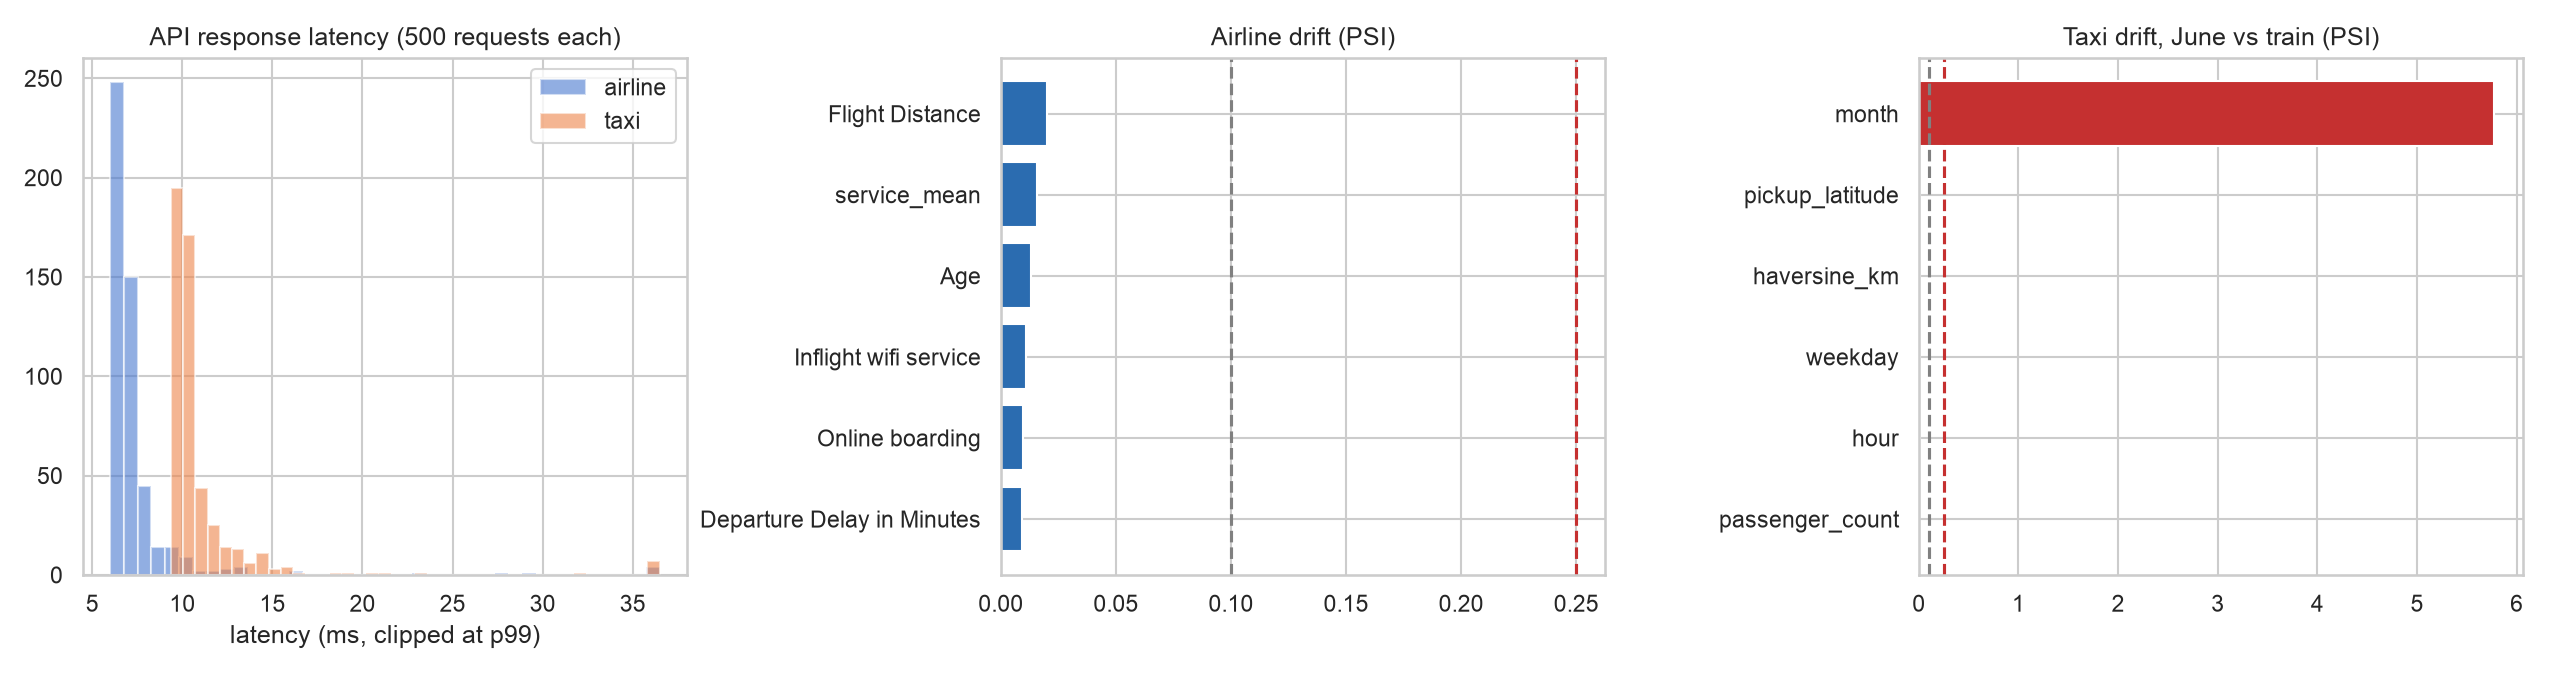
\includegraphics[width=\textwidth]{monitoring_latency_drift.png}
\caption{API latency distribution and PSI drift per feature.}
\end{figure}

\noindent The \texttt{month} feature shows significant drift (PSI \psiMonth). This is expected, because the production batch contains only June trips while the training reference covers January--June. It is exactly the signal that would trigger a scheduled retrain when new months of data arrive. All other monitored features stay stable (PSI $<$ 0.1), and live accuracy on the 500 requests matches the test results, so no retraining is needed yet. \textbf{Feedback:} the Streamlit app asks users whether a prediction was correct, or for the actual trip time, and stores the answers in \texttt{logs/feedback.csv} as labelled data for the next retraining cycle. \textbf{Maintenance plan:} retrain monthly, or when any key feature has PSI $>$ 0.25 or live RMSLE / F1 degrades by more than 5\% relative.

%=====================================================================
\section{Conclusion}

Both projects meet their success criteria on unseen test data. The airline classifier scores \airTestAccPct{} accuracy, F1 \airTestF{} and AUC \airTestRocAuc. The taxi regressor scores RMSLE \taxiTestRmsle{} (the mean baseline scores \taxiMeanBaselineValRmsle) and $R^2$ \taxiTestRtwoLog.
In both cases, gradient-boosted trees with careful cleaning and domain features outperformed linear and bagging baselines. Random search found better settings than the defaults, and validation monitoring kept the train--validation gap small.
Next steps: add weather and live-traffic data to the taxi model, use probability calibration and cost-sensitive thresholds for the airline model, and automate retraining from the monitoring signals.

\section*{Reproducibility}
\begin{lstlisting}
python3 -m venv .venv && source .venv/bin/activate && pip install -r requirements.txt
python src/airline_pipeline.py && python src/taxi_pipeline.py && python src/monitor.py
python report/make_metrics.py && cd report && latexmk -pdf report.tex
\end{lstlisting}

\end{document}
